\documentclass[11pt,a4paper]{article}
\usepackage[utf8]{inputenc}
\usepackage[margin=2.5cm]{geometry}
\usepackage{iohk}
\usepackage{microtype}
\usepackage{mathpazo} % nice fonts
\usepackage{amsmath}
\usepackage{amssymb}
\usepackage{latexsym}
\usepackage{mathtools}
\usepackage{stmaryrd}
\usepackage{extarrows}
\usepackage{slashed}
\usepackage[colon]{natbib}
\usepackage[unicode=true,pdftex,pdfa,colorlinks=true]{hyperref}
\usepackage{xcolor}
\usepackage[capitalise,noabbrev,nameinlink]{cleveref}
\usepackage{float}
\floatstyle{boxed}
\restylefloat{figure}
\usepackage{listings} % for code blocks.
%%
%% Package `semantic` can be used for writing inference rules.
%%
\usepackage{semantic}
%% Setup for the semantic package
\setpremisesspace{20pt}
\usepackage{tikz}
\usetikzlibrary{decorations.pathreplacing, positioning, arrows.meta, calc}
% For drawing simple diagrams involving arrows between LaTeX symbols
\usepackage{tikz-cd}

%%
%% Types
%%
\newcommand{\Bool}{\type{Bool}}
\newcommand{\Tx}{\type{Tx}}
\newcommand{\Ix}{\type{Ix}}
\newcommand{\TxId}{\type{TxId}}
\newcommand{\Addr}{\type{Addr}}
\newcommand{\UTxO}{\type{UTxO}}
\newcommand{\Value}{\type{Value}}
\newcommand{\Lovelace}{\type{Lovelace}}
\newcommand{\UTxOEnv}{\type{UTxOEnv}}
\newcommand{\UTxOState}{\type{UTxOState}}
%% Adding witnesses
\newcommand{\TxIn}{\type{TxIn}}
\newcommand{\TxOut}{\type{TxOut}}
\newcommand{\VKey}{\type{VKey}}
\newcommand{\SKey}{\type{SKey}}
\newcommand{\KeyHash}{\type{KeyHash}}
\newcommand{\SkVk}{\type{SkVk}}
\newcommand{\Sig}{\type{Sig}}
\newcommand{\Data}{\type{Data}}
%% Adding delegation
\newcommand{\Epoch}{\type{Epoch}}
\newcommand{\VKeyGen}{\type{VKey_G}}
%% Blockchain
\newcommand{\Gkeys}{\var{G_{keys}}}
\newcommand{\Block}{\type{Block}}
\newcommand{\CEEnv}{\type{CEEnv}}
\newcommand{\CEState}{\type{CEState}}
\newcommand{\BDEnv}{\type{BDEnv}}
\newcommand{\BDState}{\type{BDState}}
\newcommand{\Slot}{\type{Slot}}
\newcommand{\SlotCount}{\type{SlotCount}}

%%
%% Functions
%%
\newcommand{\txins}[1]{\fun{txins}~ \var{#1}}
\newcommand{\txid}[1]{\fun{txid}~ \var{#1}}
\newcommand{\txouts}[1]{\fun{txouts}~ \var{#1}}
\newcommand{\values}[1]{\fun{values}~ #1}
\newcommand{\balance}[1]{\fun{balance}~ \var{#1}}
%% UTxO witnesses
\newcommand{\inputs}[1]{\fun{inputs}~ \var{#1}}
\newcommand{\wits}[1]{\fun{wits}~ \var{#1}}
\newcommand{\verify}[3]{\fun{verify} ~ #1 ~ #2 ~ #3}
\newcommand{\sign}[2]{\fun{sign} ~ #1 ~ #2}
\newcommand{\serialised}[1]{\llbracket \var{#1} \rrbracket}
\newcommand{\addr}[1]{\fun{addr}~ \var{#1}}
\newcommand{\hash}[1]{\fun{hash}~ \var{#1}}
\newcommand{\txbody}[1]{\fun{txbody}~ \var{#1}}
\newcommand{\txfee}[1]{\fun{txfee}~ \var{#1}}
\newcommand{\minfee}[2]{\fun{minfee}~ \var{#1}~ \var{#2}}
% wildcard parameter
\newcommand{\wcard}[0]{\underline{\phantom{a}}}
%% Adding ledgers...
\newcommand{\utxo}[1]{\fun{utxo}~ #1}
%% Delegation
\newcommand{\delegatesName}{\fun{delegates}}
\newcommand{\delegates}[3]{\delegatesName~#1~#2~#3}
\newcommand{\dwho}[1]{\fun{dwho}~\var{#1}}
\newcommand{\depoch}[1]{\fun{depoch}~\var{#1}}
%% Delegation witnesses
\newcommand{\dbody}[1]{\fun{dbody}~\var{#1}}
\newcommand{\dwit}[1]{\fun{dwit}~\var{#1}}
%% Blockchain
\newcommand{\bwit}[1]{\fun{bwit}~\var{#1}}
\newcommand{\bslot}[1]{\fun{bslot}~\var{#1}}
\newcommand{\bbody}[1]{\fun{bbody}~\var{#1}}
\newcommand{\bdlgs}[1]{\fun{bdlgs}~\var{#1}}
%% Set notation
\newcommand\Set[2]{\{\,#1\mid#2\,\}}
%% Let bindings
\newcommand{\leteq}{\ensuremath{\mathrel{\mathop:}=}}

%% For properties
\newcommand{\txs}{\ensuremath{\mathcal{T}}}
\newcommand{\transtar}[2]{\xlongrightarrow[\textsc{#1}]{#2}\negthickspace^{*}}
\newcommand{\biguo}[1]{\ensuremath{\underset{#1}{\underrightarrow\bigcup}}}

%\includeonly{update-mechanism, delegation, blockchain-interface}

%% Parameters that control floats placement. See https://robjhyndman.com/hyndsight/latex-floats/
\setcounter{topnumber}{2}
\setcounter{bottomnumber}{2}
\setcounter{totalnumber}{4}
\renewcommand{\topfraction}{0.85}
\renewcommand{\bottomfraction}{0.85}
\renewcommand{\textfraction}{0.15}
\renewcommand{\floatpagefraction}{0.7}
\newcommand{\DEnv}{\type{DEnv}}
\newcommand{\DSEnv}{\type{DSEnv}}
\newcommand{\DSState}{\type{DSState}}
\newcommand{\DCert}{\type{DCert}}
\newcommand{\DState}{\type{DState}}
\newcommand{\DEState}{\type{DEState}}


\newtheorem{definition}{Definition}
\newtheorem{property}{Property}

\begin{document}

\hypersetup{
  pdftitle={A Formal Specification of the Cardano Ledger},
  breaklinks=true,
  bookmarks=true,
  colorlinks=false,
  linkcolor={blue},
  citecolor={blue},
  urlcolor={blue},
  linkbordercolor={white},
  citebordercolor={white},
  urlbordercolor={white}
}

  \cleardoublepage%
  \tableofcontents%

  \listoffigures%
  \clearpage%

  \begin{changelog}
        \change{2019/10/08}{Jared Corduan, Polina Vinogradova and Matthias G\"udemann}{FM (IOHK)}{Initial version (0.1).}
        \change{2019/10/08}{Kevin Hammond}{FM (IOHK)}{Added cover page.}
        \change{2020/11/17}{Jared Corduan}{FM (IOHK)}
          {Removed unused deliverable outline image,
           set version to 1.0,
           and changed the reward calculation so that $\eta$
             takes $d$ into account.}
        \change{2021/05/17}{Jared Corduan}{FM (IOHK)}{Added Example Illustration.}
        \change{2021/06/14}{Jared Corduan}{FM (IOHK)}
          {Added an errata section,
           fixed a typo in leader check and in the LEDGERS rule index,
           and synced the reward calculation with the implementation}
        \change{2021/06/17}{Jared Corduan}{FM (IOHK)}
          {Allow the pool influence parameter $a_0$ to be zero,
          remove all mentions of deposit decay, sync varibale names with code.}
        \change{2021/08/27}{Jared Corduan}{FM (IOHK)}{Fixed definitions in the header-only validation properties.
          CHAIN transition did not need to use previous protocol parameters.}
        \change{2021/10/08}{Jared Corduan}{FM (IOHK)}{The function createRUpd
          should get the pool parameters from the go snapshot.
          The TICKN rule was missing from the dependency diagram.}
        \change{2021/11/08}{Jared Corduan}{FM (IOHK)}{Fixed typo in the description of variable length encodings.}
        \change{2021/12/13}{Jared Corduan}{FM (IOHK)}{Re-wrote the MIR transitions to be more compact.}
      \end{changelog}
      \clearpage%
\renewcommand{\thepage}{\arabic{page}}
\setcounter{page}{1}

\title{A Formal Specification of the Cardano Ledger}

\author{Jared Corduan  \\ {\small \texttt{jared.corduan@iohk.io}} \\
   \and Polina Vinogradova \\ {\small \texttt{polina.vinogradova@iohk.io}} \\
   \and Matthias G\"udemann  \\ {\small \texttt{matthias.gudemann@iohk.io}}}

%\date{}

\maketitle

\begin{abstract}
This document provides a formal specification of the Cardano ledger for use in the upcoming Shelley implementation.
It is intended to underpin a Haskell executable specification that will be the basis of the initial
Shelley release, and represents a core design and quality assurance document.
It will be used to define properties and tests, and to provide the basis for strong formal assurance
using mathematical proof techniques.
The document defines the rules for extending the ledger with transactions
that will affect both UTxO and stake delegation.
Key properties that have been identified include the preservation of balances, absence of double spend, stakepool registration,
and reward splitting.
\end{abstract}

\section*{List of Contributors}
\label{acknowledgements}

Nicol\'as Arqueros,
Dan Bornside,
Nicholas Clarke,
Duncan Coutts,
Ruslan Dudin,
Sebastien Guillemot,
Kevin Hammond,
Vincent Hanquez,
Ru Horlick,
Michael Hueschen,
Christian Lindgren,
Yun Lu,
Philipp Kant,
Jean-Christophe Mincke,
Damian Nadales,
Ashish Prajapati,
Nicolas Di Prima,
Andrew Westberg.


\tableofcontents
\listoffigures

\chapter{Overview}
The Cardano blockchain system is based on the Ouroboros family of protocols
for a proof-of-stake cryptocurrency.
The operation of these protocols on a node, working in collaboration with the consensus
and ledger aspects of Cardano, create the overall distributed system.
It is that distributed system that defines the "single source of truth" that is the distributed ledger.
The Ouroboros papers describe these protocols in a high-level mathematical formalism
that allows for a concise presentation and is appropriate for peer review by cryptography experts.
For separation of concerns, the papers do not describe a concrete implementation of the Ouroboros
protocols.

This document has a broader scope.
It is addressed to system designers and engineers who have an IT background
but are not necessarily crypto experts,
but want to implement Cardano or to understand the reference implementation.
The description of the protocol in this document contains all the information needed to
implement the data diffusion functionality of a compatible Cardano network node.
It covers:
\begin{itemize}
\item How nodes join the network.
\item The general semantics of the messages that nodes exchange.
\item The binary format of the messages.
\item The order in which nodes send and receive the messages of the protocol.
\item The permissible protocol states for each participant in the protocol.
\end{itemize}
This information is typically found in the description of network protocols.

However, the Ouroboros proof-of-stake cryptocurrency has additional requirements,
of a sort that are not typically covered in a
protocol  description itself.
While these underlying requirements are essential for understanding the design of the protocol,
it also makes sense to also discuss these aspects and requirements in this document.
Typical network protocols describe simple information exchanges;
the distributed nature of blockchain computation means
that additional contextual information is available.
Use of this context allows, for example, for validated store and forward
which is an essential feature to contain the effect of potential malicious actions
against the distributed system.

Shelley is a first fully decentralised release of Cardano system, implementing the Ouroboros protocol.

This Chapter contains an overview of the content and scope of this document and aspects that
are being discussed.

\wip{
\subsubsection{Software assurance}
Software assurance
}

\subsubsection{Layered Protocols}
Traditionally network protocols are presented as a stack of layers where
upper layers build on services provided by lower layers and lower layers
are independent of the implementation of the upper layers.
This concept of layers is misleading when discussing Ouroboros.
For example, it is {\em not} the case that the consensus (layer)
is built on top of the network (layer).
It is more appropriate to talk about a network component than a network layer.
The network component provides services to the consensus component and vice versa;
both components rely on each other.
The network component uses the consensus component to validate
information that it distributes to other nodes, which
is essential to guard against certain kinds of DoS attacks.
Existing peer-to-peer systems focus on a slightly different problem domain.
For example, they do not consider the information validation issue
or are concerned with issues such as 'eclipse attacks' that to not
apply to the Ouroboros family of protocols.

%\missingfigure[figwidth=6cm]{Testing a long text string}

\subsubsection{Performance of the Ouroboros Network}
In computer science, Byzantine Fault Tolerance is a property of a distributed algorithm, which states
that it works for the honest participants
under the assumption that a certain proportion of the participants are indeed honest.
A similar, but more informal property applies to performance of the Ouroboros network as well.

The network provides a service to its participants while at the same
time the participants provide a service to the network.
The performance of the Ouroboros network depends (among other things) on the performance of the nodes,
while the performance of a node also depends on the performance of the network.
Not only are there honest and adversarial participant, but there is also a huge variety of
possible network topographies, bandwidths and latencies of network connections and other
factors that determine the performance of the network.

This document discusses the high level functional and performance requirements for Ouroboros and the
assumptions made about the structure of the underlying P2P network.

\subsubsection{Protocol vs Implementation}
Network Protocols are written at different levels of abstraction.
To be useful, a protocol description must be precise enough to be implemented.
A protocol description should also be abstract enough to allow alternative implementations of the protocol
and to facilitate developing and improving it.
Furthermore, it should be possible to both implement an
abstract version of a protocol
and interpret it in a real-world scenario.
For example, it must be possible to implement a protocol
such that the real-world software runs on a machine with a typical size of memory
and a typical speed network connection.

The Shelley network protocol design has been developed in parallel
with a reference implementation in Haskell.
Haskell (more precisely GHC) has built-in support for high level concurrency abstractions
such as light-weight threads and software transactional memory.
While the protocol itself is completely language agnostic, it still makes sense to discuss some
aspects of the Haskell reference implementation in this document.
In particular, the document describes how to achieve good resource bounds for
a protocol implementation.

\wip{
  \subparagraph{Threats}
  Reference the Threats section.
  'eclipse' can be deterred}


\wip{TODO:extended abstract, scope of the document}

\section{High level requirements and User Stories}

These are the high level business requirements for the networking that were
gathered and signed off in late 2017. As such they are expressed in informal
prose, often following a ``user story'' style.
Roughly, there are three different kinds of users:
\begin{itemize}
\item Users who have delegated.
\item Small stakeholders.
\item Large stakeholders.
\end{itemize}

\subsubsection{Network connectivity}\label{network-connectivity}

\paragraph{Participate as a user who has delegated}

As a Daedalus home user with my stake delegated to other users
I would like to join the Cardano network so I can participate in the network.
\begin{itemize}
\item The system must be designed to provide this user segment with the ability
      to catch up and keep up with the blockchain without having
      to do any local network configuration.
\item The system must be designed to provide this user segment with the ability to
      continuously find and maintain a discovery of a sufficient number of
      other network participants that have reasonable connectivity.
\item The system must be designed to provide this user segment with the ability to
      find and maintain a minimum of 3 other network participants to maintain
      connectivity with performance that is sufficient to catch up with the
      blockchain.
\item The system design will take into account that this user will probably be
      behind a firewall.
\item Users in the segment can be defined by having all their stake
      delegated to other network participants.
      As such they will never be selected as a slot leader (i.e required to generate a block).
\end{itemize}


\paragraph{Participate in network as small stakeholder}

As a Daedalus home user operating a node with a small stake,
I would like to join the Cardano network so I can participate in the network as a
node that produces blocks i.e. my stake is not delegated to someone else.

\begin{itemize}
\item The system must be designed to provide this user segment with the ability to
      receive the transactions that will be incorporated into blocks (although
      sizing the operation of the distributed system to ensure that all such
      participants would be able to receive all transactions is not a bounding
      constraint).
\item The system must be designed to provide this user segment with the ability to
      participate in the MPC protocol\footnote{This requirement is now
      redundant because the MPC protocol is specific to Ouroboros Classic.}.
\item The system will be designed to provide this user segment with the ability
      to catch up and keep up with the blockchain without having to do any local
      network configuration (this is a bounding constraint).
\item The user will have sufficient connectivity and performance to receive a
      block within a time slot {\sc and} they have to be able to create and
      broadcast a block within a time slot in which the block is received by
      other participating nodes.
\item The system will be designed to maximise the likelihood that 50\% of home
      users operating a participating node are compliant with the previous requirement
      at any one time.
\item The system will be designed to provide this user segment with the ability
      to continuously find and maintain a discovery of a sufficient number of
      other network participants that have reasonable connectivity.
\item The system will provide a discovery mechanism that will find and maintain
      a minimum of 3 other network participants to maintain connectivity with
      performance that is sufficient to catch up with the blockchain.
\item The system design will take into account that this user may be behind a
      firewall (i.e being behind a firewall should not preclude a user
      participating in this fashion).
\item The Delegation work stream will provide a UI feature for the user to
      choose to control their own stake.
\item Users in this segment will be defined as {\sc not}
      \begin{itemize}
      \item[a)] being in the top 100 users ranked by stake or
      \item[b)] in a ranked set of users who together control 80\% of the stake
      \end{itemize}
\item Users in this segment will not be part of the Core Dif, but still
      subject to the normal incentives related to creating blocks.
\end{itemize}


\paragraph{Participate in network as a large stakeholder}

As a user running a core node on a server and with large stake in the network,
I would like to join the Cardano network so I can participate in the network as
a core server node that produces blocks i.e. have not delegated to someone else.

\begin{itemize}
\item A large stakeholder will be defined as
      \begin{itemize}
      \item[a)] being in the top 100 users ranked by stake; or
      \item[b)] in a ranked set of users who combined control 80\% of the stake
      \end{itemize}
\item Assuming that this user has sufficient connectivity and performance, the
      system should ensure that the collective operation of the distributed
      system will ensure that they have a high probability of receiving a
      block within a time slot such that they have sufficient time to be able
      to create and broadcast a block within a time slot where the block is
      received by other core nodes.
\item It is expected that the previous requirement will be fulfilled to a high
      degree of reliability between nodes in this category -- assuming normal
      network operations

      \begin{tabular}{rl}
      Threshold & $>95\%$ \\
      Target    & $>98\%$ \\
      Stretch   & $>99\%$
      \end{tabular}
\item The system will be designed to provide this user segment with the ability
      to continuously find and maintain a discovery of a sufficient number of
      other network participants that have reasonable connectivity.
\item Discovery will find and maintain a minimum of 10 other network
      participants to maintain connectivity with performance that is sufficient
      to catch up with the blockchain.
\item Ability to receive the transactions that will be incorporated into blocks.
\item Ability to participate in the MPC protocol\footnote{This requirement is
      now redundant because the MPC protocol is specific to Ouroboros Classic.}.
\item The user will catch up and keep up with the blockchain.
\item The server firewall rules will be such that it can communicate with other
      core nodes on the system (and vice versa) -- The system will provide the
      necessary information to update firewall rules if the server is operating
      behind a firewall to ensure the server can communicate with other core
      nodes.
\item The threshold which defines the group of large stakeholders may be
      configurable on the network layer. The configuration may include toggling
      between the rules a) and b) in the previous requirement and the threshold
      numbers within these (this is pending a decision from the Incentives
      work stream.
\item The rules and threshold configuration may need to be a protocol parameter
      that is updated by the update system.
\end{itemize}


\paragraph{Poor network connectivity notification}

As a home user, I want to see a network connection status on Daedalus so that
I know the state of my network connection.
%
\begin{itemize}
\item If the user receives a notification that they are in red or amber mode,
      Daedalus will give the user some helpful information on how to resolve
      common connectivity issues.
\end{itemize}
%
There are three (at least) the following three distinct modes that the network can be operating in:
each one has a red, green, amber status.

%
\begin{center}
\begin{tabular}{ll}
Initial block sync \\
\hline
red   & receiving $<1$ blocks per 10s \\
amber & receiving $<10$ blocks per 10s \\
green & otherwise  \\[1em]

Recovery \\
\hline
red   & receiving $<1$ block per 10s \\
amber & otherwise  \\
green & (not applicable) \\[1em]

Block chain following \\
\hline
red   & it has been more that 200s since a slot indication was received. \\
amber & it has been more than 60s since a slot indication was received. \\
green & otherwise.
\end{tabular}
\end{center}

This assumes that the slot time remains 20 seconds, or at least that the average time
between production of new blocks is 20 seconds.

\paragraph{Transaction Latency}

As a user I want my transaction to be submitted to the blockchain and received
by the target user within the following time period:
%
\begin{center}
\begin{tabular}{lr}
Threshold & 100 seconds \\
Target    & 60 seconds  \\
Stretch   & 30 seconds  \\
\end{tabular}
\end{center}
%
The above time-frames will be achieved for $>95\%$ of all transactions.

\paragraph{Network Bearer Resource Use -- end user control}

As a user operating on the network as a home user not behind a firewall, I
would like a cap on the total amount of network capacity in terms of short-term
bandwidth that other network users can request from my connection so I am
assured my network resource is not eaten up by the data diffusion function.

\begin{itemize}
\item The cap should be based on a fraction of a typical home internet
      connection -- it can be changed by configuration including ``don't act
      as a super node''.
\item The system will allow users syncing with the latest version of the
      blockchain to download blocks from more then one and up to five network
      peers concurrently.
\item A cap on number of incoming subscribers.
\item A cap on number of outbound requests for block syncing from other users.
\item The cap will not be imposed on core nodes running on a server.
\item If these resources are available, a reasonable connection speed should be
      available to users requesting to sync the latest version of the
      blockchain e.g. downloading blocks from 5 peers concurrently to aggregate
      the bandwidth.
\item (nice to have) the actual number and capacity being used is available to
      user.
\end{itemize}

\paragraph{Participant performance measurement}

There may be a requirement for measuring if a large stakeholder is not meeting
their network obligation \cite{DBLP:journals/corr/abs-1807-11218}.

It is accepted that this requirement is a ``nice to have'', and it has not been
established that it is possible, nor has it been incorporated into the
incentives mechanism.

\subsubsection{Distributed System Resilience and Security}

\paragraph{Resilience to abuse}

As a user I should not be able to attack the system using an asymmetric denial
of service attack that will deplete network resources from other users.

\begin{itemize}
\item The system should achieve its connectivity and performance requirements
      even in the presence of a non-trivial proportion of bad actors on the
      network.
\item There is an assumption that there are not a large numbers of bad actors
      in the network.
\item The previous assumption does not follow from the assumptions of Ouroboros
      which states that the users that control 50\% of the stake are
      non-adversarial.
\end{itemize}


\paragraph{DDoS protection}

As a large stakeholder running a core node on a server, I should still be able
to communicate with other user in this segment, even if the system comes under
a DDoS attack.

\begin{itemize}
\item Users in this segment will be able to generate and broadcast blocks to
      each other within the usual timing constraints in this situation.
\end{itemize}

IP addresses will be hidden.

\begin{itemize}
\item Encrypted IP addresses will be published by 10 of the other members of
      the group of large stakeholder core nodes.
\end{itemize}

Assumption

\begin{itemize}
\item Core node operators will not publish their IP addresses publicly.
\item Encrypted IP addresses will be published by the 10 of the other members
      of the group of large stakeholder core nodes.
\item If a node operator's IP address is compromised the operator will respond
      and change the IP address of their node.
\item The system will allow operators to change the address of their core nodes
      and communicate with that new IP address within a reasonable period of
      time.
\end{itemize}


\subsubsection{Network decentralisation}

\paragraph{No hegemony}

As a user I want to be assured that IOHK and its business partners are not in
an especially privileged position in terms of trust, responsibility and
necessity to the network so that network hegemony is avoided.

\begin{itemize}
\item IOHK should be in the same position on the network as any other
      stakeholder with an equivalent amount of stake.
\item There is a more general requirement that no other actor could
      achieve hegemonic control of the operation of the data diffusion layer.
\end{itemize}


\wip{
\section{Context and Introduction}

How this work relates (in general terms) to the rest of the Shelley
development and the Ouroboros papers.

\subsection{Data Diffusion assumptions in Ouroboros}
\begin{quote}
  This is the ``telling them what you are going to tell them'' part -
  outline of the data diffusion and overlay network bringing out the
  key functional and non-functional relationships - aim to serve as a
  general executive overview as well as a framing of PoS issues.
\end{quote}
\begin{itemize}
  \item Assumptions of the mathematical model(s)
  \item Goal of the data diffusion functionality
  \item Strong requirement on collective performance
  \begin{itemize}
    \item Chain growth quality
    \item Adversarial actor assumption
  \end{itemize}
\end{itemize}
\subsection{Functional Layering}
\hide[inline]{pictures as to how the various functional layers relate; How the Data
diffusion layer relates to Ledger etc; How data diffusion relates to
point-to-point overlay network.}

\subsubsection{Non-function aspects}
Performance; trustworthiness; Forwarding as an expression of confirmed
``trust'' (and corollary - forwarding of \emph{clearly} incorrect information
seen as prima-facie evidence of adversarial action.
\subsection{Protocol Roles}
Peer relationship between various nodes; Limited trust and
verification; (Brief) description of the expectations and assumptions across
the functionality boundaries;
}

\wip{
\subsubsection{Mini Protocols}
\begin{description}
\item[Chain Sync]
\item[Block Fetch]
\item[Transaction Submission]
\item[$\Delta Q$ Measurement] (not really a mini protocol, in that it
  is point-to-point and not part of the diffusion process itself,
  placed here because it ``sits'' on top of the overlay network. Role
  to generate active endpoint performance data to help optimise
  time-to-diffuse critical information exchanges (e.g. newly minted
  block diffusion)
\end{description}
}
\wip{
\subsubsection{Point-to-point Overlay Network}
\hide[inline]{need a picture} Note that long term eclipse attacks are not an issue
here (cover why a bit later); tie in chain growth requirements with
need for ``better'' communications performance between (major)
stake pools (notion of Core DIF); association explain need for
\begin{itemize}
\item fixed configuration (with/without others from this list)
\item Core DIF
\item Distributed endpoint discovery (subset of notion of peer in
  other approaches)
\end{itemize}
}

\wip{
\section{Layout of the Document}

\begin{itemize}
  \item What goes in which section ?
  \item In which order to read ?
  \item Which sections can be skipped ?
\end{itemize}

\section{Notation}
}

\wip{
\chapter{Requirements}

\section{Performance Requirements and User Stories}
\subsection{Classes of Participants}
\wip{todo: make a nice table}
\hide{Some information about participants is in the previous
section~\ref{network-connectivity}}

\subsubsection{Stake pool} % lookup what this is called in the protocols.tex
\subsubsection{Small stakeholder}
\subsubsection{User who has delegated}
\subsubsection{Requirements for Participants}
\subsubsection{Requirements for Stake Pools}
\subsubsection{Services that the System should provide}

There are two kinds of Requirements:

\begin{enumerate}
\item System capabilities for a node to take a blockchain slot creation role in the protocol.
\item What services that the system provides to the user.
\end{enumerate}

}

\hide{
\section{Protocol Updates on the Blockchain}
\begin{itemize}
\item Hybrid phase of federation and decentralisation
\item Gradually transition between protocol variants on a live blockchain.
\item Several protocol variants active in parallel, version negotiation.
\item Communication between Shelley Nodes and existing core nodes.
\item Byron proxy
\end{itemize}

\section{Node to Node and Node to Consumer IPC}
There are two basic variants of inter-process-communication in the network:
\begin{itemize}
\item IPC between Cardano nodes that are engaged in the high level Ouroboros
      blockchain consensus protocol.
\item IPC between a Cardano node and a `chain consumer' component such as a
      wallet, explorer or other custom application.
\end{itemize}
Both variants of IPC in the network follow distinct requirements and constraints, and
,while the first version of Cardano used a single protocol, the new version will
use different sets of protocols for both uses cases.
(See Section~\ref{why_distinguish_protocols} for the motivation for this design decision.)
Throughout the document it will be clear which variant of we are referring to.

\section{Threat Model}

\wip{
  WIP discussion of the threat model
\subsection{Resource Consumption Attacks}
}
}
\hide{
\section{Ouroboros}
\wip{
How PoS is different from PoW in its network requirements:
}

\begin{itemize}
  \item No capability to sustain an undetected Eclipse attack
  \item Sustained liveness requirement
\end{itemize}

\section{Delegation}
}

\chapter{System Architecture}
\hide{
\section{Overview}
This section describes the key underlying aspects and considerations of the design
of the network protocol and tries to give a big picture the overall network protocol.

\section{Key Functionality}

\wip{
  Here only an outline. Full discussion in the Section~\ref{ouroboros}.
\begin{description}
\item[Block diffusion]
\item[Chain following]
\item[Forwarding transactions]
\end{description}
}

\section{High Assurance Software}
\wip{How does the software/protocol design reflect the high assurance requirements ?}

\section{Modular Design and Mini Protocols}
\wip{Why are mini protocols a good idea ?}
\wip{How does polymorphism help modularity ?}
}

\section{Congestion Control}
A central design goal of the system is robust operation at high workloads.
For example, it is a normal working condition of the networking design
that transactions arrive at a higher rate than the number
that can be included in blockchain.
An increase of the rate at which transactions are submitted must not cause a decrease
of the block chain quality.

Point-to-point TCP bearers do not deal well with overloading.
A TCP connection has a certain maximal bandwidth,
i.e. a certain maximum load that it can handle relatively reliably under normal conditions.
If the connection is ever overloaded,
the performance characteristics will degrade rapidly unless
the load presented to the TCP connection is appropriately managed.


At the same time, the node itself has a limit on the rate at which it can process data.
In particular, a node may have to share its processing power with other processes that run on the
same machine/operation system instance, which means that a node may get slowed down for some reason,
and the system may get in a situation
where there is more data available from the network than the node can process.
The design must operate appropriately in this situation and recover form transient conditions.
In any condition, a node must not exceed its memory limits,
that is there must be defined limits, breaches of which being treated like protocol violations.

Of cause it makes no sense if the system design is robust,
but so defensive that it fails to meet performance goals.
An example would be a protocol that never transmits a message unless it has received an
explicit ACK for the previous message. This approach might avoid overloading the network,
but would waste most of the potential bandwidth.

\hide{
\subsection{Back Pressure}
Back Pressure is a strategy for congestion control for push based buffered channels like
,for example, TCP connections.



\wip{TODO: explain the concept of Back pressure and how it is used in the design}
\subsection{Push vs Pull}
\wip{TODO: data flow inside the node is pull based}
\subsection{Delta Q}
\wip{TODO: explain what delta Q means and what it has to do with congestion control.}
}

\begin{figure}[ht]
  \pgfdeclareimage[height=15cm]{node-diagram-chains-state}{figure/node-diagram-chains-state.pdf}
  \begin{center}
    \pgfuseimage{node-diagram-chains-state}
  \end{center}
  \caption{Data flow inside a Node}
  \label{node-diagram-concurrency}
\end{figure}

\section{Data Flow in a Node}
Nodes maintain connections with the peers that have been chosen
with help of the peer selection process.
Suppose node $A$ is connected to node $B$.
The Ouroboros protocol schedules a node $N$ to generate a new block in a given time slot.
Depending on the location of nodes $A$, $B$ and $N$ in the network topology and whether the new
block arrives first at $A$ or $B$, $A$ can be either up-stream or down-stream of $B$.
Therefore, node $A$ runs an instance of the client side of the chain-sync mini protocol
that talks with a server instance of chain-sync at node $B$ and also a server instance of chain sync
that talks with a client instance at $B$.
The situation is similar for the other mini protocols (block fetch, transaction submission, etc).
The set of mini protocols that runs over a connection is determined by the version of the network
protocol, i.e.  Node-to-Node, Node-to-Wallet and Node-to-Chain-Consumer
connections use different sets of mini protocols (e.g. different protocol
versions).  The version is negotiated when a new connection is established
using protocol which is described in Chapter~\ref{connection-management}.
\hide{Add description of this protocol in Chapter~\ref{connection-management}
and link it.}

Figure~\ref{node-diagram-concurrency} illustrates parts of the data flow in a node.
Circles represents a thread that runs one of the mini protocols (the mini protocols are explained in
Chapter~\ref{state-machine-section}).
There are two kinds of data flows:
mini protocols communicate with mini protocols of other nodes by sending and receiving messages;
and, within a node, they communicate by reading from- and writing to- a shared
mutable state (represented by boxes in Figure~\ref{node-diagram-concurrency}).
\href{https://en.wikipedia.org/wiki/Software_transactional_memory}{Software transactional memory}
(STM) is a mechanism for safe and lock-free concurrent
access to mutable state and the reference implementation makes intensive use of this abstraction.

\section{Real-time Constraints and Coordinated Universal Time}
Ouroboros models the passage of physical time as an infinite sequence of time slots,
i.e. contiguous, equal-length intervals of time,
and assigns slot leaders (nodes that are eligible to create a new block) to those time slots.
At the beginning of a time slot, the slot leader selects the block chain and transactions that are the basis
for the new block, then it creates the new block and sends the new block to its peers.
When the new block reaches the next block leader before the beginning of next time slot,
the next block leader can extend the block chain upon this block (if the block
did not arrive on time the next leader will create a new block anyway).

There are some trade-offs when choosing the slot time that is used for the protocol but
basically the slot length should be long enough such that a new block has a good chance to reach the
next slot leader in time.
A chosen value for the slot length is 20 seconds.
It is assumed that the clock skews between the local clocks of the nodes is small with respect to the
slot length.

However, no matter how accurate the local clocks of the nodes are with respect to the time slots
the effects of a possible clock skew must still be carefully considered.
For example, when a node time-stamps incoming blocks with its local clock time, it may encounter
blocks that are created in the future
with respect to the local clock of the node.
The node must then decide whether this is because of a clock skew or whether the node considers this
as adversarial behaviour of an other node.

\wip{TODO :: get feedback from the researchers on this. Tentative policy: allow 200ms to 1s
explain the problem in detail.
A node cannot forward a block from the future.
}


\section{Notation}

In addition to the notation in the Shelley spec, we use the following notations:

\begin{description}
\item[Functions with finite support] For a monoid $M$, $A \to_0 M$
  are the functions $f : A \to M$ with finite support, i.e. such that
  there exist only finitely many $a \in A$ such that $f a \neq 0$. We
  denote the support of $f$ by $\supp f$, which is defined as
  $\supp f := \{ a \in A : f a \neq 0 \}$.
\end{description}


\section{Cryptographic primitives}
\label{sec:crypto-primitives}

Figure~\ref{fig:crypto-defs} introduces the cryptographic abstractions used in
this document. Note that we define a family of serialization functions
$\serialised{\wcard}_\type{A}$, for all types $\type{A}$ for which such
serialization function can be defined. When the context is clear, we omit the
type suffix, and use simply $\serialised{\wcard}$.

\begin{figure}[htb]
  \emph{Abstract types}
  %
  \begin{equation*}
    \begin{array}{r@{~\in~}lr}
      \var{vk} & \SKey & \text{signing key}\\
      \var{vk} & \VKey & \text{verifying key}\\
      \var{hk} & \KeyHash & \text{hash of a key}\\
      \sigma & \Sig  & \text{signature}\\
      \var{d} & \Data  & \text{data}\\
    \end{array}
  \end{equation*}
  \emph{Derived types}
  \begin{equation*}
    \begin{array}{r@{~\in~}lr}
      (sk, vk) & \SkVk & \text{signing-verifying key pairs}
    \end{array}
  \end{equation*}
  \emph{Abstract functions}
  %
  \begin{equation*}
    \begin{array}{r@{~\in~}lr}
      \hash{} & \VKey \to \KeyHash
      & \text{hash function} \\
      %
      \fun{verify} & \VKey \times \Data \times \Sig
      & \text{verification relation}\\
      \serialised{\wcard}_\type{A} & \type{A} \to \Data
      & \text{serialization function for values of type $\type{A}$}\\
      \fun{sign} & \SKey \to \Data \to \Sig
      & \text{signing function}
    \end{array}
  \end{equation*}
  \emph{Constraints}
  \begin{align*}
    & \forall (sk, vk) \in \SkVk,~ m \in \Data,~ \sigma \in \Sig \cdot
      \sign{sk}{m} = \sigma \Rightarrow \verify{vk}{m}{\sigma}
  \end{align*}
  \emph{Notation}
  \begin{align*}
    & \mathcal{V}^\sigma_{\var{vk}}~{d} = \verify{vk}{d}{\sigma}
      & \text{shorthand notation for } \fun{verify}
  \end{align*}
  \caption{Cryptographic definitions}
  \label{fig:crypto-defs}
\end{figure}

\subsection{A note on serialization}
\label{sec:a-note-on-serialization}

\begin{definition}[Distributivity over serialization functions]
  For all types $\type{A}$ and $\type{B}$, given a function
  $\fun{f} \in \type{A} \to \type{B}$, we say that the serialization function
  for values of type $\type{A}$, namely $\serialised{ }_\type{A}$ distributes
  over $\fun{f}$ if there exists a function $\fun{f}_{\serialised{ }}$ such
  that for all $a \in \type{A}$:
  \begin{equation}
    \label{eq:distributivity-serialization}
    \serialised{\fun{f}~a}_\type{B} = \fun{f}_{\serialised{ }}~\serialised{a}_\type{A}
  \end{equation}
\end{definition}
The equality defined in \cref{eq:distributivity-serialization} means that the
following diagram commutes:

\[
  \begin{tikzcd}
    A \arrow{r}{\fun{f}} \arrow{d}{\serialised{ }_\type{A}}
    & B \arrow{d}{\serialised{ }_\type{B}} \\
    \Data \arrow{r}{\fun{f}_{\serialised{ }}} & \Data
  \end{tikzcd}
\]

Throughout this specification, whenever we use
$\serialised{\fun{f}~a}_\type{B}$, for some type $\type{B}$ and function
$\fun{f} \in \type{A} \to \type{B}$, we assume that $\serialised{ }_\type{A}$
distributes over $\fun{f}$ (see for example
Rule~\ref{eq:utxo-witness-inductive}). This property is what allow us to
extract a component of the serialized data (if it is available) without
deserializing it in the cases in which the deserialization function
($\serialised{\wcard}^{-1}_\type{A}$) doesn't behave as an inverse of
serialization:

\begin{equation*}
  \serialised{\wcard}^{-1}_\type{A} \cdot \serialised{\wcard}_\type{A} \neq \fun{id}_\type{A}
\end{equation*}

For the cases in which such an inverse exists, given a function $\fun{f}$, we
can readily define $\fun{f}_{\serialised{ }}$ as:

\begin{equation*}
  \fun{f}_{\serialised{ }} \dot{=} \serialised{\wcard}_\type{B}
                            . \fun{f}
                            . \serialised{\wcard}^{-1}_\type{A}
\end{equation*}


\section{UTxO}
\label{sec:utxo}

Some of the functions related to scripts, datums and collateral need
to be adjusted for the new features. Most of these adjustments are
self-explanatory. Note that the new $\fun{collOuts}$ function
generates a single output with an index $| \txouts{txb} |$. This is to
avoid potential confusion for transactions spending that output. Note
that $\TxId$ can only hold integers up to $2^{16} - 1$. In case of an
overflow, we let this number be $2^{16} - 1$.

\begin{figure*}[htb]
  \emph{Functions}
  %
  \begin{align*}
    & \fun{isTwoPhaseScriptAddress} : \Tx \to \hldiff{\UTxO} \to \Addr \to \Bool \\
    & \fun{isTwoPhaseScriptAddress}~tx~\hldiff{utxo}~a = \\
    &\quad\begin{cases}
        \True  & a \in \AddrScr \land \fun{validatorHash}~a \mapsto s \in \fun{txscripts}~tx~\hldiff{utxo} \land s \in \ScriptPhTwo \\
        \False & \text{otherwise}
      \end{cases}
    \nextdef
    & \fun{collOuts} : \TxBody \to \UTxO \\
    & \fun{collOuts}~txb =
      \begin{cases}
        \emptyset                                                      & \fun{collRet}~txb = \Nothing \\
        \{ (\txid{txb}, | \txouts{txb} |) \mapsto \fun{collRet}~txb \} & \text{otherwise}
      \end{cases}
    \nextdef
    & \fun{collBalance} : \TxBody \to \UTxO \to \Value \\
    & \fun{collBalance}~txb~utxo = \fun{ubalance}~(\var{utxo}|_{\fun{collInputs}~{txb}}) - \fun{ubalance}~(\fun{collOuts}~txb)
    \nextdef
    & \fun{feesOK} : \PParams \to \Tx \to \UTxO \to \Bool  \\
    & \fun{feesOK}~\var{pp}~tx~utxo = \\
    &~~      \minfee{pp}{tx} \leq \txfee{tx} \wedge (\fun{txrdmrs}~tx \neq \Nothing \Rightarrow \\
    &~~~~~~~~~~\forall (a, \wcard, \wcard) \in \fun{range}~(\fun{collInputs}~tx \restrictdom \var{utxo}), a \in \AddrVKey \\
    &~~~~~~\wedge \fun{adaOnly}~\var{balance} \\
    &~~~~~~\wedge \var{balance} \geq \hldiff{\lceil \txfee{txb} * \fun{collateralPercent}~pp / 100 \rceil} \\
    &~~~~~~\wedge \hldiff{(\fun{txcoll}~tx \neq \Nothing) \Rightarrow \var{balance} = \fun{txcoll}~tx} \\
    &~~~~~~\wedge \fun{collInputs}~{tx} \neq \emptyset) \\
    &~~      \where \\
    & ~~~~~~~ \var{balance}=\hldiff{\fun{collBalance}~tx~utxo}
  \end{align*}
  \caption{Functions related to fees and collateral}
  \label{fig:functions:utxo}
\end{figure*}

\begin{figure*}
  \begin{align*}
    & \fun{getDatum} : \Tx \to \UTxO \to \ScriptPurpose \to \seqof{\Datum} \\
    & \fun{getDatum}~{tx}~{utxo}~{sp} =
      \begin{cases}
        [\var{d}] & \var{sp} \in \TxIn, (\_, \_, h, \_) \in \var{utxo}~\var{sp},~ \var{d}\in\fun{txdats}~(\fun{txwits}~tx)~\var{h} \\
        [\var{d}] & \hldiff{\var{sp} \in \TxIn, (\_, \_, d, \_) \in \var{utxo}~\var{sp},~ \var{d} \in \Datum} \\
        \epsilon  & \text{otherwise}
      \end{cases}
    \nextdef
    & \fun{refScripts} : \Tx \to \hldiff{\UTxO} \to \ScriptHash \pto \Script \\
    & \fun{refScripts}~tx~utxo = \{ \fun{hash}~s \mapsto s \mid (\_, \_, \_, s) \in \var{utxo}~(\fun{spendInputs}~tx \cup \fun{refInputs}~tx)\}
    \nextdef
    & \fun{txscripts} : \Tx \to \hldiff{\UTxO} \to \ScriptHash \pto \Script \\
    & \fun{txscripts}~tx~utxo = \fun{txwitscripts}~tx \cup \hldiff{\fun{refScripts}~tx~utxo}
    \nextdef
    & \fun{allOuts} : \Tx \to \powerset{\TxOut} \\
    & \fun{allOuts}~tx = \range \txouts{tx} \cup \fun{collRet}~tx
    \nextdef
    & \fun{languages} : \Tx \to \UTxO \to \powerset{\Language} \\
    & \fun{languages}~tx~utxo =
      \{\fun{language}~s \mid s \in \range (\fun{txscripts}~tx~\hldiff{utxo}) \cap \ScriptPhTwo\}
    \nextdef
    & \fun{allowedLanguages} : \Tx \to \UTxO \to \powerset{\Language} \\
    & \fun{allowedLanguages}~tx~utxo = \\
    & \begin{cases}
        \emptyset                   & \text{if}~\exists (a, \_, \_, \_) \in os, a \in \AddrBS \\
        \{ \PlutusVII \}            & \text{if}~\exists (\_, \_, d, s) \in os, d \in \Datum \lor s \neq \Nothing \lor \fun{refInputs}~tx \neq \emptyset \\
        \{ \PlutusVI, \PlutusVII \} & \text{otherwise}
      \end{cases} \\
    & \where \var{os} = \range \txouts{tx} \cup \var{utxo}~(\fun{spendInputs}~tx \cup \fun{refInputs}~tx)
  \end{align*}
  \caption{Functions related to scripts}
  \label{fig:functions:data}
\end{figure*}

\begin{figure}[htb]
  \begin{equation}
    \inference[Scripts-Yes]
    {
    \var{txb}\leteq\txbody{tx} &
    \var{sLst} := \fun{collectTwoPhaseScriptInputs}~\var{pp}~\var{tx}~\var{utxo}
    \\~\\
    {
      \begin{array}{r}
        \var{slot} \\
        \var{pp} \\
        \var{genDelegs} \\
      \end{array}
    }
    \vdash \var{pup} \trans{\hyperref[fig:rules:update]{ppup}}{\fun{txup}~\var{tx}} \var{pup'}
    \\~\\
    \var{refunded} \leteq \keyRefunds{pp}{txb}
    \\
    \var{depositChange} \leteq
      \fun{totalDeposits}~{pp}~\var{poolParams}~(\txcerts{txb})~-~\var{refunded}
    \\~\\
    \fun{isValid}~\var{tx} = \fun{evalScripts}~\var{tx}~\var{sLst} = \True
    }
    {
    \begin{array}{l}
      \var{slot}\\
      \var{pp}\\
      \var{poolParams}\\
      \var{genDelegs}\\
    \end{array}
      \vdash
      \left(
      \begin{array}{r}
        \var{utxo} \\
        \var{deposits} \\
        \var{fees} \\
        \var{pup} \\
      \end{array}
      \right)
      \trans{utxos}{tx}
      \left(
      \begin{array}{r}
        \varUpdate{\var{(\fun{spendInputs}~txb \subtractdom \var{utxo}) \cup \outs{txb}}}  \\
        \varUpdate{\var{deposits} + \var{depositChange}} \\
        \varUpdate{\var{fees} + \txfee{txb}} \\
        \varUpdate{\var{pup'}} \\
      \end{array}
      \right) \\
    }
  \end{equation}
  \begin{equation}
    \inference[Scripts-No]
    {
    \var{txb}\leteq\txbody{tx} &
    \var{sLst} := \fun{collectTwoPhaseScriptInputs}~\var{pp}~\var{tx}~\var{utxo} \\
    \hldiff{\var{collateralFees} := \fun{valueToCoin}~(\fun{collBalance}~txb~utxo)}
    \\
    ~
    \\
    \fun{isValid}~\var{tx} = \fun{evalScripts}~\var{tx}~\var{sLst} = \False
    }
    {
    \begin{array}{l}
      \var{slot}\\
      \var{pp}\\
      \var{poolParams}\\
      \var{genDelegs}\\
    \end{array}
      \vdash
      \left(
      \begin{array}{r}
        \var{utxo} \\
        \var{deposits} \\
        \var{fees} \\
        \var{pup} \\
      \end{array}
      \right)
      \trans{utxos}{tx}
      \left(
      \begin{array}{r}
        \varUpdate{\var{(\fun{collInputs}~{txb} \subtractdom \var{utxo})} \cup \hldiff{\fun{collOuts}~txb}}  \\
        \var{deposits} \\
        \varUpdate{\var{fees} + \hldiff{\var{collateralFees}}} \\
        \var{pup} \\
      \end{array}
      \right)
    }
  \end{equation}
  \caption{State update rules}
  \label{fig:rules:utxo-state-upd}
\end{figure}

\begin{figure}[htb]
  \begin{equation}
    \inference[UTxO-inductive]
    {
      \var{txb}\leteq\txbody{tx} &
      \fun{ininterval}~\var{slot}~(\fun{txvldt}~{txb}) &
      \var{(\wcard, i_f)}\leteq\fun{txvldt}~{tx} \\~\\
      \Nothing \notin \{\fun{txrdmrs}~\var{tx}, i_f\} \Rightarrow \fun{epochInfoSlotToUTCTime}~\mathsf{EI}~\mathsf{SysSt}~i_f \neq \Nothing \\
      \fun{spendInputs}~txb \neq \emptyset
      & \fun{feesOK}~pp~tx~utxo
      \\
      \fun{spendInputs}~txb \cup \fun{collInputs}~txb \cup \hldiff{\fun{refInputs}~{tx}} \subseteq \dom \var{utxo} \\
      \consumed{pp}{utxo}{txb} = \produced{pp}{poolParams}~{txb}
      \\~\\
      \mathsf{adaID}\notin \supp {\fun{mint}~tx} \\~\\
      \forall txout \in \hldiff{\fun{allOuts}~txb}, \\
      \fun{getValue}~txout \geq \fun{inject}~(\hldiff{\lceil\fun{serSize}~txout * \fun{coinsPerUTxOWord}~pp/8\rceil}) \\~
      \\
      \forall txout \in \hldiff{\fun{allOuts}~txb},\\
      \fun{serSize}~(\fun{getValue}~txout) \leq \fun{maxValSize}~pp \\~
      \\
      \forall (\wcard\mapsto (a,~\wcard)) \in \hldiff{\fun{allOuts}~txb}, a \in \AddrBS \Rightarrow \fun{bootstrapAttrsSize}~a \leq 64 \\
      \forall (\wcard\mapsto (a,~\wcard)) \in \hldiff{\fun{allOuts}~txb}, \fun{netId}~a = \NetworkId
      \\
      \forall (a\mapsto\wcard) \in \txwdrls{txb}, \fun{netId}~a = \NetworkId \\
      (\fun{txnetworkid}~\var{txb} = \NetworkId) \vee (\fun{txnetworkid}~\var{txb} = \Nothing)
      \\~\\
      \fun{txsize}~{tx}\leq\fun{maxTxSize}~\var{pp} \\~\\
      \fun{totExunits}~{tx} \leq \fun{maxTxExUnits}~{pp} &  \| \fun{collInputs}~{tx} \| \leq \fun{maxCollateralInputs}~{pp}
      \\
      ~
      \\
      {
        \begin{array}{c}
          \var{slot}\\
          \var{pp}\\
          \var{poolParams}\\
          \var{genDelegs}\\
        \end{array}
      }
      \vdash
      {
        \left(
          \begin{array}{r}
            \var{utxo} \\
            \var{deposits} \\
            \var{fees} \\
            \var{pup}\\
          \end{array}
        \right)
      }
      \trans{utxos}{\var{tx}}
      {
        \left(
          \begin{array}{r}
            \var{utxo'} \\
            \var{deposits'} \\
            \var{fees'} \\
            \var{pup'}\\
          \end{array}
        \right)
      }
    }
    {
      \begin{array}{l}
        \var{slot}\\
        \var{pp}\\
        \var{poolParams}\\
        \var{genDelegs}\\
      \end{array}
      \vdash
      \left(
      \begin{array}{r}
        \var{utxo} \\
        \var{deposits} \\
        \var{fees} \\
        \var{pup}\\
      \end{array}
      \right)
      \trans{utxo}{tx}
      \left(
      \begin{array}{r}
        \varUpdate{\var{utxo'}}  \\
        \varUpdate{\var{deposits'}} \\
        \varUpdate{\var{fees'}} \\
        \varUpdate{\var{pup'}}\\
      \end{array}
      \right)
    }
  \end{equation}
  \caption{UTxO inference rules}
  \label{fig:rules:utxo-babbage}
\end{figure}

To the UTXOW rule, in addition to the changes required by the new
features, we add a check that all scripts and datums involved in the
transaction are well-formed. Also, we forbid transactions that use the
new features and try to use $\PlutusVI$ scripts.

\begin{figure}
  \begin{equation}
    \label{eq:utxo-witness-inductive-babbage}
    \inference[UTxO-witG]
    {
      \var{txb}\leteq\txbody{tx} &
      \var{txw}\leteq\fun{txwits}~{tx} \\
      (utxo, \wcard, \wcard, \wcard) \leteq \var{utxoSt} \\
      \var{witsKeyHashes} \leteq \{\fun{hashKey}~\var{vk} \vert \var{vk} \in
      \dom (\txwitsVKey{txw}) \}\\
      \var{inputHashes}\leteq \left\{ h \,\middle|
        {
          \begin{array}{l}
            (a, \_, h) \in \range(\var{utxo}|_{\fun{spendInputs}~tx}) \\
            \fun{isTwoPhaseScriptAddress}~tx~\hldiff{utxo}~a \\
          \end{array}
        }
      \right\} - \hldiff{\Datum} \\~\\
      \forall \var{s} \in \range (\fun{txscripts}~txw~\hldiff{utxo}) \cap \ScriptPhOne,
      \fun{validateScript}~\var{s}~\var{tx}\\~\\
      \{ h \mid (\_, h) \in \fun{scriptsNeeded}~\var{utxo}~txb\} - \hldiff{\dom (\fun{refScripts}~tx~utxo)} = \dom (\fun{txwitscripts}~txw) \\~\\
      \var{inputHashes} \subseteq_{\{h \mid (\wcard, \wcard, h)\in\fun{allOuts}~tx \cup \hldiff{\var{utxo}~(\fun{refInputs}~{tx})}\}} \dom (\fun{txdats}~{txw})  \\~\\
      \\~\\
      \dom (\fun{txrdmrs}~tx) = \left\{ \fun{rdptr}~txb~sp \,\middle|
        {
          \begin{array}{l}
            (sp,h) \in \fun{scriptsNeeded}~\var{utxo}~txb \\
            \fun{txscripts}~{txw}~\hldiff{utxo}~h \in \ScriptPhTwo
          \end{array}
        } \right\}
      \\~\\
      \var{txbodyHash}\leteq\fun{hash}~(\txbody{tx}) \\
      \forall \var{vk} \mapsto \sigma \in \txwitsVKey{tx},
      \mathcal{V}_{\var{vk}}{\serialised{txbodyHash}}_{\sigma} \\
      \fun{witsVKeyNeeded}~{utxo}~{tx}~{genDelegs} \subseteq witsKeyHashes
      \\~\\
      genSig \leteq
      \left\{
        \fun{hashKey}~gkey \vert gkey \in\dom{genDelegs}
      \right\}
      \cap
      \var{witsKeyHashes}
      \\
      \left\{
        c\in\txcerts{txb}~\cap\DCertMir
      \right\} \neq\emptyset \implies \vert genSig\vert \geq \Quorum
      \\~\\
      \var{adh}\leteq\fun{txADhash}~\var{txb}
      &
      \var{ad}\leteq\fun{auxiliaryData}~\var{tx}
      \\
      (\var{adh}=\Nothing \land \var{ad}=\Nothing)
      \lor
      (\var{adh}=\fun{hashAD}~\var{ad})
      \\~\\
      \hldiff{\forall x \in \range (\fun{txdats}~txw) \cup \range (\fun{txwitscripts}~txw)} \\
      \hldiff{\cup \bigcup_{(\_, \_, d, s) \in \hldiff{\fun{allOuts}~txb}} \{s, d\} \cup \fun{scripts}~(\fun{auxiliaryData}~tx),} \\
      \hldiff{x \in \Script \cup \Datum \Rightarrow \fun{isWellFormed}~x}
      \\~\\
      \fun{languages}~tx~\hldiff{utxo} \subseteq \dom(\fun{costmdls}~pp) \cap \fun{allowedLanguages}~tx~utxo \\
      \fun{scriptIntegrityHash}~{txb} =
      \fun{hashScriptIntegrity}~\var{pp}~(\fun{languages}~{txw}~\hldiff{utxo})~(\fun{txrdmrs}~{txw})~(\fun{txdats}~{txw})
      \\~\\
      {
        \begin{array}{r}
          \var{slot}\\
          \var{pp}\\
          \var{poolParams}\\
          \var{genDelegs}\\
        \end{array}
      }
      \vdash \var{utxoSt} \trans{\hyperref[fig:rules:utxo-shelley]{utxo}}{tx}
      \var{utxoSt'}\\
    }
    {
      \begin{array}{r}
        \var{slot}\\
        \var{pp}\\
        \var{poolParams}\\
        \var{genDelegs}\\
      \end{array}
      \vdash \var{utxoSt} \trans{utxow}{tx} \varUpdate{\var{utxoSt'}}
    }
  \end{equation}
  \caption{UTxO with witnesses inference rules for Tx}
  \label{fig:rules:utxow-babbage}
\end{figure}


\section{Delegation}
\label{sec:delegation}

An agent owning a key that can sign new blocks can delegate its signing rights
to another key by means of \textit{delegation certificates}. These certificates
are included in the ledger, and therefore also included in the body of the
blocks in the blockchain.

There are several restrictions on a certificate posted on the blockchain:
\begin{enumerate}
\item Only genesis keys can delegate.
\item Certificates must be properly signed by the delegator.
\item Any given key can delegate at most once per-epoch.
\item Any given key can issue at most one certificate in a given slot.
\item The epochs in the certificates must refer to the current or to the next
  epoch. We do not want to allow certificates from past epochs so that a
  delegation certificate cannot be replayed. On the other hand if we allow
  certificates with arbitrary future epochs, then a malicious key can issue a
  delegation certificate per-slot, setting the epoch to a sufficiently large
  value. This will cause a blow up in the size of the ledger state since we
  will not be able to clean $\var{eks}$ (we only clean past epochs). Also note
  that we do not check the relation between the certificate epoch and the slot
  in which the certificate becomes active. This would bring additional
  complexity without any obvious benefit.
\item Certificates do not become active immediately, but they require a certain
  number of slots till they become stable in all the nodes.
\end{enumerate}
These conditions are formalized in \cref{fig:rules:delegation-scheduling}.
Rule~\ref{eq:rule:delegation-scheduling} determines when a certificate can
become ``scheduled''. The definitions used in these rules are presented in
\cref{fig:defs:delegation-scheduling}, and the types of the system induced by
$\trans{sdeleg}{\wcard}$ are presented in
\cref{fig:ts-types:delegation-scheduling}. Here and in the remaining rules we
will be using $k$ as an abstract constant that gives us the chain stability
parameter.

\begin{figure}[htb]
  \emph{Abstract types}
  \begin{equation*}
    \begin{array}{r@{~\in~}lr}
      c & \DCert & \text{delegation certificate}\\
      \var{vk_g} & \VKeyGen & \text{genesis verification key}\\
    \end{array}
  \end{equation*}

  \emph{Derived types}
  \begin{equation*}
    \begin{array}{r@{~\in~}l@{\qquad=\qquad}r@{~\in~}lr}
      \var{e} & \Epoch & n & \mathbb{N} & \text{epoch}\\
      \var{s} & \Slot & s & \mathbb{N} & \text{slot}\\
      \var{d} & \SlotCount & s & \mathbb{N} & \text{slot}
    \end{array}
  \end{equation*}

  \emph{Constraints}
  \begin{align*}
    \VKeyGen \subseteq \VKey
  \end{align*}

  \emph{Abstract functions}
  \begin{equation*}
    \begin{array}{r@{~\in~}lr}
      \fun{dbody} & \DCert \to (\VKey \times \Epoch)
      & \text{body of the delegation certificate}\\
      \fun{dwit} & \DCert \to (\VKeyGen \times \Sig)
      & \text{witness for the delegation certificate}\\
      \fun{dwho} & \DCert \mapsto (\VKeyGen \times \VKey)
      & \text{who delegates to whom in the certificate}\\
      \fun{depoch} & \DCert \mapsto \Epoch
      & \text{certificate epoch}\\
      \var{k} & \mathbb{N} & \text{chain stability parameter}
    \end{array}
  \end{equation*}
  \caption{Delegation scheduling definitions}
  \label{fig:defs:delegation-scheduling}
\end{figure}

\begin{figure}[htb]
  \emph{Delegation scheduling environments}
  \begin{equation*}
    \DSEnv =
    \left(
      \begin{array}{r@{~\in~}lr}
        \mathcal{K} & \powerset{\VKeyGen} & \text{allowed delegators}\\
        \var{e} & \Epoch & \text{epoch}\\
        \var{s} & \Slot & \text{slot}\\
      \end{array}
    \right)
  \end{equation*}

  \emph{Delegation scheduling states}
  \begin{equation*}
    \DSState
    = \left(
      \begin{array}{r@{~\in~}lr}
        \var{sds} & \seqof{(\Slot \times (\VKeyGen \times \VKey))} & \text{scheduled delegations}\\
        \var{eks} & \powerset{(\Epoch \times \VKeyGen)} & \text{key-epoch delegations}
      \end{array}
    \right)
  \end{equation*}

  \emph{Delegation scheduling transitions}
  \begin{equation*}
    \var{\_} \vdash
    \var{\_} \trans{sdeleg}{\_} \var{\_}
    \subseteq \powerset (\DSEnv \times \DSState \times \DCert \times \DSState)
  \end{equation*}
  \caption{Delegation scheduling transition-system types}
  \label{fig:ts-types:delegation-scheduling}
\end{figure}

\begin{figure}[htb]
  \begin{equation}
    \label{eq:sdeleg-bootstrap}
    \inference
    {
      \var{sds_0} \leteq \epsilon
      &
      \var{eks_0} \leteq \emptyset
    }
    {
      {\left(\begin{array}{l}
       \mathcal{K}\\
        e\\
        s
      \end{array}\right)}
      \vdash
      \trans{sdeleg}{}
      \left(
        \begin{array}{l}
          \var{sds_0}\\
          \var{eks_0}
        \end{array}
      \right)
    }
  \end{equation}
  \nextdef
  \begin{equation}
    \label{eq:rule:delegation-scheduling}
    \inference
    {
      (\var{vk_s},~ \sigma) \leteq \dwit{c}
      & \verify{vk_s}{\serialised{\dbody{c}}}{\sigma} & vk_s \in \mathcal{K}\\ ~ \\
      (\var{vk_s},~ \var{vk_d}) \leteq \dwho{c} & e_d \leteq \depoch{c}
      & (e_d,~ \var{vk_s}) \notin \var{eks} & 0 \leq e_d - e \leq 1 \\ ~ \\
      d \leteq 2 \cdot k & (s + d,~ (\var{vk_s},~ \wcard)) \notin \var{sds}\\
    }
    {
      {\left(\begin{array}{l}
       \mathcal{K}\\
        e\\
        s
      \end{array}\right)}
      \vdash
      {
        \left(
          \begin{array}{l}
            \var{sds}\\
            \var{eks}
          \end{array}
        \right)
      }
      \trans{sdeleg}{c}
      {
        \left(
          \begin{array}{l}
            \var{sds}; (s + d,~ (\var{vk_s},~ \var{vk_d}))\\
            \var{eks} \cup \{(e_d,~ \var{vk_s})\}
          \end{array}
        \right)
      }
    }
  \end{equation}
  \caption{Delegation scheduling rules}
  \label{fig:rules:delegation-scheduling}
\end{figure}

\clearpage

The rules in Figure~\ref{fig:rules:delegation} model the activation of
delegation certificates. Once a scheduled certificate becomes active
(see~\cref{sec:delegation-interface-rules}), the delegation map is changed by
it only if:
\begin{itemize}
\item The delegating key ($\var{vk_s}$) did not activate a delegation
  certificate in a slot greater or equal than the certificate slot ($s$). This
  check is performed to avoid having the constraint that the delegation
  certificates have to be activated in slot order.
\item The key being delegated to ($\var{vk_d}$) has not been delegated by
  another key (injectivity constraint).
\end{itemize}
The reason why we check that the delegation map is injective is to avoid a
potential risk (during the OBFT era) in which a malicious node gets control of
a genesis key $\var{vk_m}$ that issued the maximum number of blocks in a given
window. By delegating to another key $\var{vk_d}$, which was already delegated to
by some other key $\var{vk_g}$, the malicious node could prevent $\var{vk_g}$
from issuing blocks. Even though the delegation certificates take several slots
to become effective, the malicious node could calculate when the certificate
would become active, and issue a delegation certificate at the right time.

As an additional advantage, by having an injective delegation map, we are able
to simplify our specification when it comes to counting the blocks issued by
(delegates of) genesis keys.

Note also, that we could not impose the injectivity constraint in
Rule~\ref{eq:rule:delegation-scheduling} since we do not have information about
the delegations that will become effective. We could of course detect a
violation in the injectivity constraint when scheduling a delegation
certificate, but this will lead to a complex computation and larger state in
said rule.

Finally, note that we do not want to reject a scheduled delegation that would
violate the injectivity constraint (since delegation might not have been
scheduled by the node issuing the block). Instead, we simply ignore the
delegation certificate (Rule~\ref{eq:rule:delegation-nop}).

\begin{figure}[htb]
  \begin{align*}
    & \unionoverrideRight \in (A \mapsto B) \to (A \mapsto B) \to (A \mapsto B)
    & \text{union override}\\
    & d_0 \unionoverrideRight d_1 = d_1 \cup (\dom d_1 \subtractdom d_0)
  \end{align*}
  \caption{Functions used in delegation rules}
  \label{fig:funcs:delegation}
\end{figure}

\begin{figure}[htb]
  \emph{Delegation environments}
  \begin{equation*}
    \DEnv =
    \left(
      \begin{array}{r@{~\in~}lr}
        \mathcal{K} & \powerset{\VKeyGen} & \text{allowed delegators}
      \end{array}
    \right)
  \end{equation*}

  \emph{Delegation states}
  \begin{align*}
    & \DState
      = \left(
        \begin{array}{r@{~\in~}lr}
          \var{dms} & \VKeyGen \mapsto \VKey & \text{delegation map}\\
          \var{dws} & \VKeyGen \mapsto \Slot & \text{when last delegation occurred}\\
        \end{array}\right)
  \end{align*}
  \emph{Delegation transitions}
  \begin{equation*}
    \_ \vdash \_ \trans{adeleg}{\_} \_ \in
    \powerset (\DEnv \times \DState \times (\Slot \times (\VKeyGen \times \VKey)) \times \DState)
    \end{equation*}
  \caption{Delegation transition-system types}
  \label{fig:ts-types:delegation}
\end{figure}

\begin{figure}[htb]
  \begin{equation}
    \label{eq:adeleg-bootstrap}
    \inference
    {
      \var{dms_0} \leteq \Set{k \mapsto k}{k \in \mathcal{K}} &
      \var{dws_0} \leteq \Set{k \mapsto 0}{k \in \mathcal{K}}
    }
    {
      \left(
        \mathcal{K}
      \right)
      \vdash
      \trans{adeleg}{}
      \left(
        \begin{array}{l}
          \var{dms_0}\\
          \var{dws_0}
        \end{array}
      \right)
    }
  \end{equation}
  \nextdef
  \begin{equation}\label{eq:rule:delegation-change}
    \inference
    {
      \var{vk_d} \notin \range~\var{dms} & (\var{vk_s} \mapsto s_p \in \var{dws} \Rightarrow s_p < s)
    }
    {
      \left(\mathcal{K}\right)
      \vdash
      \left(
      \begin{array}{r}
        \var{dms}\\
        \var{dws}
      \end{array}
      \right)
      \trans{adeleg}{(s,~ (vk_s,~ vk_d))}
      \left(
      \begin{array}{lcl}
        \var{dms} & \unionoverrideRight & \{\var{vk_s} \mapsto \var{vk_d}\}\\
        \var{dws} & \unionoverrideRight & \{\var{vk_s} \mapsto s \}
      \end{array}
      \right)
    }
  \end{equation}
  \nextdef
  \begin{equation}\label{eq:rule:delegation-nop}
    \inference
    {\var{vk_d} \in \range~\var{dms} \vee (\var{vk_s} \mapsto s_p  \in \var{dws}  \wedge s \leq s_p)
    }
    {
      \left(\mathcal{K}\right)
      \vdash
      \left(
      \begin{array}{r}
        \var{dms}\\
        \var{dws}
      \end{array}
      \right)
      \trans{adeleg}{(s,~ (\var{vk_s},~ \var{vk_d}))}
      \left(
      \begin{array}{lcl}
        \var{dms}\\
        \var{dws}
      \end{array}
      \right)
    }
  \end{equation}
  \caption{Delegation inference rules}
  \label{fig:rules:delegation}
\end{figure}

\clearpage

\subsection{Delegation sequences}
\label{sec:delegation-sequences}

This section presents the rules that model the effect that sequences of
delegations have on the ledger.

\begin{figure}[htb]
  \begin{equation}
    \inference
    {
      {\begin{array}{l}
         \var{delegEnv}
      \end{array}}
      \vdash
      \trans{\hyperref[eq:sdeleg-bootstrap]{sdeleg}}{}
      \var{delegSt}
    }
    {
      {\begin{array}{l}
         \var{delegEnv}
      \end{array}}
      \vdash
      \trans{sdelegs}{}
      \var{delegSt}
    }
  \end{equation}
  \nextdef
  \begin{equation}
    \label{eq:rule:delegation-scheduling-seq-base}
    \inference
    {}
    {
      \var{delegEnv}
      \vdash
      \var{delegSt}
      \trans{sdelegs}{\epsilon}
      \var{delegSt}
    }
  \end{equation}
  \nextdef
  \begin{equation}
    \label{eq:rule:delegation-scheduling-seq-ind}
    \inference
    {
      \var{delegEnv}
      \vdash
      \var{delegSt}
      \trans{sdelegs}{\Gamma}
      \var{delegSt'}
      &
      \var{delegEnv}
      \vdash
      \var{delegSt'}
      \trans{\hyperref[fig:rules:delegation-scheduling]{sdeleg}}{c}
      \var{delegSt''}
    }
    {
      \var{delegEnv}
      \vdash
      \var{delegSt}
      \trans{sdelegs}{\Gamma; c}
      \var{delegSt''}
    }
  \end{equation}
  \caption{Delegation scheduling sequence rules}
  \label{fig:rules:delegation-scheduling-seq}
\end{figure}

\begin{figure}
  \begin{equation}
    \inference
    {
      {\begin{array}{l}
         \var{delegEnv}
      \end{array}}
      \vdash
      \trans{\hyperref[eq:adeleg-bootstrap]{adeleg}}{}
      \var{delegSt}
    }
    {
      {\begin{array}{l}
         \var{delegEnv}
      \end{array}}
      \vdash
      \trans{adelegs}{}
      \var{delegSt}
    }
  \end{equation}
  \nextdef
  \begin{equation}
    \label{eq:rule:delegation-seq-base}
    \inference
    {}
    {
      \var{delegEnv}
      \vdash
      \var{delegSt}
      \trans{adelegs}{\epsilon}
      \var{delegSt}
    }
  \end{equation}
  \nextdef
  \begin{equation}
    \label{eq:rule:delegation-seq-ind}
    \inference
    {
      \var{delegEnv}
      \vdash
      \var{delegSt}
      \trans{adelegs}{\Gamma}
      \var{delegSt'}
      &
      \var{delegEnv}
      \vdash
      \var{delegSt'}
      \trans{\hyperref[fig:rules:delegation]{adeleg}}{c}
      \var{delegSt''}
    }
    {
      \var{delegEnv}
      \vdash
      \var{delegSt}
      \trans{adelegs}{\Gamma; c}
      \var{delegSt''}
    }
  \end{equation}
  \caption{Delegations sequence rules}
  \label{fig:rules:delegation-seq}
\end{figure}

\subsection{Deviation from the \texttt{cardano-sl} implementation}
\label{sec:delegation:deviation-cardano-sl-imp}

In the \texttt{cardano-sl} implementation, the block issuer needs to include a
delegation certificate in the block, which witness the fact that a genesis key
gave the issuer the rights of issuing blocks on behalf of this genesis key. The
reasons why this was implemented in this way in \texttt{cardano-sl} are not
clear, since the delegation certificates are posted on the chain, so the ledger
state contains the information about who delegates to whom. Hence in the
current specification we use a heavyweight delegation scheme, i.e. where the
certificates are posted on the chain, but an implementation of this rules that
aims at being compatible with the implementation in \texttt{cardano-sl} has to
take the fact that delegation certificates are also present in a block into
account.


\newcommand{\UProp}{\ensuremath{\type{UProp}}}
\newcommand{\UPropId}{\ensuremath{\type{UpId}}}
\newcommand{\UPropSD}{\ensuremath{\type{UpSD}}}
\newcommand{\ProtVer}{\ensuremath{\type{ProtVer}}}
\newcommand{\ProtPm}{\ensuremath{\type{Ppm}}}
\newcommand{\Rpus}{\ensuremath{\type{Rpus}}}
\newcommand{\UPVEnv}{\ensuremath{\type{UPVEnv}}}
\newcommand{\UPVState}{\ensuremath{\type{UPVState}}}
\newcommand{\UPLEnv}{\ensuremath{\type{UPLEnv}}}
\newcommand{\UPLState}{\ensuremath{\type{UPLState}}}
\newcommand{\UPREnv}{\ensuremath{\type{UPREnv}}}
\newcommand{\UPRState}{\ensuremath{\type{UPRState}}}
\newcommand{\Vote}{\ensuremath{\type{Vote}}}
\newcommand{\VREnv}{\ensuremath{\type{VREnv}}}
\newcommand{\VRState}{\ensuremath{\type{VRState}}}
\newcommand{\VEnv}{\ensuremath{\type{VEnv}}}
\newcommand{\VState}{\ensuremath{\type{VState}}}
\newcommand{\BVREnv}{\ensuremath{\type{BVREnv}}}
\newcommand{\BVRState}{\ensuremath{\type{BVRState}}}
\newcommand{\ApName}{\ensuremath{\type{ApName}}}
\newcommand{\SWVer}{\ensuremath{\type{SWVer}}}
\newcommand{\ApVer}{\ensuremath{\type{ApVer}}}
\newcommand{\Metadata}{\ensuremath{\type{Mdt}}}
\newcommand{\STag}{\ensuremath{\type{STag}}}

\newcommand{\upSize}[1]{\ensuremath{\fun{upSize}~\var{#1}}}
\newcommand{\upPV}[1]{\ensuremath{\fun{upPV}~\var{#1}}}
\newcommand{\upId}[1]{\ensuremath{\fun{upId}~\var{#1}}}
\newcommand{\upSig}[1]{\ensuremath{\fun{upSig}~\var{#1}}}
\newcommand{\upSigData}[1]{\ensuremath{\fun{upSigData}~\var{#1}}}
\newcommand{\upIssuer}[1]{\ensuremath{\fun{upIssuer}~\var{#1}}}
\newcommand{\upParams}[1]{\ensuremath{\fun{upParams}~\var{#1}}}
\newcommand{\upSwVer}[1]{\ensuremath{\fun{upSwVer}~\var{#1}}}
\newcommand{\upMetadata}[1]{\ensuremath{\fun{upMdt}~\var{#1}}}
\newcommand{\vCaster}[1]{\ensuremath{\fun{vCaster}~\var{#1}}}
\newcommand{\vPropId}[1]{\ensuremath{\fun{vPropId}~\var{#1}}}
\newcommand{\vSig}[1]{\ensuremath{\fun{vSig}~\var{#1}}}

\lstset{ frame=tb,
       , language=Haskell
       , basicstyle=\footnotesize\ttfamily,
       , keywordstyle=\color{blue!80},
       , commentstyle=\itshape\color{purple!40!black},
       , identifierstyle=\bfseries\color{green!40!black},
       , stringstyle=\color{orange},
       }

\lstMakeShortInline[columns=fixed]`

\section{Update mechanism}
\label{sec:update}

This section formalizes the update mechanism by which the protocol parameters
get updated. This formalization is a simplification of the current update
mechanism implemented in
\href{https://github.com/input-output-hk/cardano-sl/}{\texttt{cardano-sl}}, and
partially documented in:
\begin{itemize}
\item \href{https://cardanodocs.com/technical/updater/}{Updater implementation}
\item \href{https://cardanodocs.com/cardano/update-mechanism/}{Update mechanism}
\item
  \href{https://github.com/input-output-hk/cardano-sl/blob/2a19d8ce2941b8e60f0208a5198943ec2ada1fd4/docs/block-processing/us.md}{Update system consensus rules}
\end{itemize}

The reason for formalizing a simplified version of the current implementation
is that research work on blockchain update mechanisms is needed before
introducing a more complex update logic. Since this specification is to be
implemented in a federated setting, some of the constraints put in place in the
current implementation are no longer relevant. Once the research work is ready,
this specification can be extended to incorporate the research results.

\subsection{Update proposals}
\label{sec:update-proposals}

The definitions used in the update mechanism rules are presented in
\cref{fig:defs:update-proposals}. A system tag is used to identify the system
for which the update is proposed (in practice this would be a string referring
to an operating system; e.g. `linux`, `win64`, or `mac32`). The software update
metadata ($\Metadata$) is any information required for performing an update
such as hashes of software downloads. Note that the fact that the metadata is
kept abstract in the specification does not mean that we allow any arbitrary
metadata (in the actual implementation this abstract metadata would correspond
to `Map SystemTag UpdateData`, were the `SystemTag` corresponds with $\STag$
and `UpdateData` contains the software hash for a specific platform).

\begin{figure}[htb]
  \emph{Abstract types}
  %
  \begin{equation*}
    \begin{array}{r@{~\in~}lr}
      \var{up} & \UProp & \text{update proposal}\\
      \var{p} & \ProtPm & \text{protocol parameter}\\
      \var{upd} & \type{UpdData} & \text{update data}\\
      \var{upa} & \type{UpdAttrs} & \text{update attributes}\\
      \var{an} & \ApName & \text{application name}\\
      \var{t} & \STag & \text{system tag}\\
      \var{m} & \Metadata & \text{metadata}
    \end{array}
  \end{equation*}
  %
  \emph{Derived types}
  \begin{equation*}
    \begin{array}{r@{~\in~}l@{~=~}r@{~\in~}lr}
      \var{s_n} & \Slot & n & \mathbb{N} & \text{slot number}\\
      \var{pv} & \ProtVer & (\var{maj}, \var{min}, \var{alt})
      & (\mathbb{N}, \mathbb{N}, \mathbb{N}) & \text{protocol version}\\
      \var{pps} & \PPMMap & \var{pps} & \ProtPm \mapsto \Value
                                         & \text{protocol parameters map}\\
      \var{apv} & \ApVer & n & \mathbb{N}\\
      \var{swv} & \SWVer
      & (\var{an}, \var{av}) & \ApName \times \ApVer
      & \text{software version}\\
      \var{pb} & \UPropSD
      &
        {\left(\begin{array}{r l}
                 \var{pv}\\
                 \var{pps}\\
                 \var{swv}\\
                 \var{upd}\\
                 \var{upa}\\
               \end{array}\right)}
      & {
        \left(
        \begin{array}{l}
          \ProtVer\\
          \PPMMap\\
          \type{SWVer}\\
          \type{UpdData}\\
          \type{UpdAttrs}\\
        \end{array}
                   \right)
                   }
               & \text{protocol update signed data}
    \end{array}
  \end{equation*}
  \emph{Abstract functions}
  %
  \begin{equation*}
    \begin{array}{r@{~\in~}lr}
      \fun{upIssuer} & \UProp \to \VKey & \text{update proposal issuer (delegate)}\\
      \fun{upSize} & \UProp \to \mathbb{N} & \text{update proposal size}\\
      \fun{upPV} & \UProp \to \ProtVer & \text{update proposal protocol version}\\
      \fun{upId} & \UProp \to \UPropId & \text{update proposal id}\\
      \fun{upParams} & \UProp \to \mathbb{\PPMMap}
                                           & \text{proposed parameters update}\\
      \fun{upSwVer} & \UProp \to \SWVer & \text{software-version update proposal}\\
      \fun{upSig} & \UProp \to \Sig & \text{update proposal signature}\\
      \fun{upSigData} & \UProp \to \UPropSD & \text{update proposal signed data}\\
      \fun{upSTags} & \UProp \to \powerset{\STag} & \text{update proposal system tags}\\
      \fun{upMdt} & \UProp \to \Metadata & \text{software update metadata}
    \end{array}
  \end{equation*}
  \caption{Update proposals definitions}
  \label{fig:defs:update-proposals}
\end{figure}

The set of protocol parameters ($\ProtPm$) is assumed to contain the following
keys, some of which correspond with fields of the
\href{https://github.com/input-output-hk/cardano-sl/}{\texttt{cardano-sl}}
`BlockVersionData` structure:
\begin{itemize}
\item Maximum block size: $\var{maxBlockSize}$
\item Maximum transaction size: $\var{maxTxSize}$
\item Maximum header size: $\var{maxHeaderSize}$
\item Maximum proposal size: $\var{maxProposalSize}$
\item Transaction fee policy: $\var{txFeePolicy}$
\item Script version: $\var{scriptVersion}$
\item Update adoption threshold: $\var{upAdptThd}$. This represents the minimum
  percentage of the total number of genesis keys that have to endorse a protocol
  version to be able to become adopted. We use this parameter to determine the
  confirmation threshold as well. There is no corresponding parameter in the
  `cardano-sl` protocol parameters, however we do have a soft-fork minimum
  threshold parameter (`srMinThd` in `bvdSoftforkRule`). When divided by,
  $1\times 10^{15}$, it determines the minimum portion of the total stake that
  is needed for the adoption of a new protocol version. On mainnet, this number
  is set to $6 \times 10^{14}$, so the minimum portion becomes $0.6$. This
  number can be multiplied by the total number of genesis keys to obtain how
  many keys are needed to reach a majority.
\item Update proposal time-to-live: $\var{upropTTL}$. This would correspond to
  the number of slots specified by `bvdUpdateImplicit`. In `cardano-sl` the
  rule was that after `bvdUpdateImplicit` slots, if a proposal did not reach a
  majority of the votes, then if the proposal has more votes for than against
  it, then it will become implicitly accepted, or rejected otherwise. In this
  specification, we re-interpret the meaning of this parameter as the proposal
  time-to-live: if after the number of slots specified by `bvdUpdateImplicit`
  the proposal does not reach a majority of approvals, the proposal is simply
  discarded. In the mainnet configuration (`mainnet-genesis.json`) this value is
  set to $10000$, which corresponds with almost half of the total number of
  slots in an epoch.
\end{itemize}

The protocol parameters are formally defined in \cref{fig:prot-params-defs}.

\begin{figure}[ht]
  \begin{equation*}
    \begin{array}{r@{~\in~}lr}
      \var{maxBlockSize} \mapsto \mathbb{N} & \PPMMap & \text{maximum block size}\\
      \var{maxTxSize} \mapsto \mathbb{N} & \PPMMap & \text{maximum transaction size}\\
      \var{maxHeaderSize} \mapsto \mathbb{N} & \PPMMap & \text{maximum header size}\\
      \var{scriptVersion} \mapsto \mathbb{N} & \PPMMap & \text{script version}\\
      \var{upAdptThd} \mapsto \mathbb{Q} & \PPMMap & \text{update proposal adoption threshold}\\
      \var{upropTTL} \mapsto \mathbb{\Slot} & \PPMMap & \text{update proposal time-to-live}\\
    \end{array}
  \end{equation*}
  \caption{Protocol-parameters definitions}
  \label{fig:prot-params-defs}
\end{figure}

\subsection{Update proposals registration}
\label{sec:update-proposals-registration}

\begin{figure}[htb]
  \emph{Update proposals validity environments}
  \begin{equation*}
    \UPVEnv =
    \left(
      \begin{array}{r@{~\in~}lr}
        \var{pv} & \ProtVer & \text{adopted (current) protocol version}\\
        \var{pps} & \PPMMap & \text{adopted protocol parameters map}\\
        \var{avs} & \ApName \mapsto (\ApVer \times \Slot \times \Metadata)
        & \text{application versions}\\
      \end{array}
    \right)
  \end{equation*}
  %
  \emph{Update proposals validity states}
  \begin{align*}
    & \UPVState \\
    & = \left(
      \begin{array}{r@{~\in~}lr}
        \var{rpus} & \UPropId \mapsto (\ProtVer \times \PPMMap)
        & \text{registered protocol update proposals}\\
        \var{raus} & \UPropId \mapsto (\ApName \times \ApVer \times \Metadata)
        & \text{registered software update proposals}\\
      \end{array}
    \right)
  \end{align*}
  %
  \emph{Update proposals validity transitions}
    \begin{equation*}
    \var{\_} \vdash
    \var{\_} \trans{upv}{\_} \var{\_}
    \subseteq \powerset (\UPVEnv \times \UPVState \times \UProp \times \UPVState)
  \end{equation*}
  \caption{Update proposals validity transition-system types}
  \label{fig:ts-types:up-validity}
\end{figure}

The rules in Figure~\ref{fig:rules:up-validity} model the validity of a proposal:
\begin{itemize}
\item if an update proposal proposes a change in the protocol version, it must
  do so in a consistent manner:
  \begin{itemize}
  \item The proposed version must be lexicographically bigger than the
    current version.
  \item The major versions of the proposed and current version must differ in
    at most one.
  \item If the proposed major version is equal to the current major
    version, then the proposed minor version must be incremented by one.
  \item If the proposed major version is larger than the current major version,
    then the proposed minor version must be zero.
  \item must be consistent with the current protocol parameters:
    \begin{itemize}
    \item the proposal size must not exceed the maximum size specified by the
      current protocol parameters, (note that here we use function application
      to extract the value of the different protocol parameters, and a rule
      that uses a value of the map can be applied only if the function -e.g.
      $\var{pps}$- is defined for that value)
    \item the proposed new maximum block size should be not greater than twice
      current maximum block size,
    \item the maximum transaction size must be smaller than the maximum block
      size (this requirement is \textbf{crucial} for having every transaction
      fitting in a block, and
    \item the proposed new script version can be incremented by at most 1.
    \end{itemize}
  \item must have a unique version among the current active proposals.
  \end{itemize}
\item if an update proposal proposes to increase the application version
  version ($\var{av}$) for a given application ($\var{an}$), then there should
  not be an active update proposal that proposes the same update.
\end{itemize}
Note that the rules in Figure~\ref{fig:rules:up-validity} allow for an update
that does not propose changes in the protocol version, or does not propose
changes to the software version. However the update proposal must contain a change
proposal in any of these two aspects.
%
Also note that we do not allow for updating the protocol parameters without
updating the protocol version. If an update in the protocol parameters does not
cause a soft-fork we might use the alt version for that purpose.

In Rule~\ref{eq:rule:up-av-validity} we make use of the following abstract
functions:
\begin{itemize}
\item $\fun{apNameValid}$, which checks that the name is an ASCII string 12
  characters or less.
\item $\fun{sTagValid}$, which checks that the name is an ASCII string of 10
  characters or less.
\end{itemize}

\begin{figure}[htb]
  \emph{Abstract functions}
  \begin{equation*}
    \begin{array}{r@{~\in~}lr}
      \fun{apNameValid} & \ApName \rightarrow \mathbb{B} & \text{validity checking for application name}\\
      \fun{sTagValid} & \STag \rightarrow \mathbb{B} & \text{validity checking for system tag}
    \end{array}
  \end{equation*}
  \caption{Update proposal validity definitions}
  \label{fig:defs:update-proposal-validity}
\end{figure}

\begin{figure}[htb]
  \begin{equation}
    \label{eq:func:pv-can-follow}
    \begin{array}{r c l}
      \fun{pvCanFollow}~(\var{mj_p}, \var{mi_p}, \var{a_p})~(\var{mj_n}, \var{mi_n}, \var{a_n})
      & = & (\var{mj_p}, \var{mi_p}, \var{a_p}) < (\var{mj_n}, \var{mi_n}, \var{a_n})\\
      & \wedge & 0 \leq \var{mj_n} - \var{mj_p} \leq 1\\
      & \wedge & (\var{mj_p} = \var{mj_n} \Rightarrow \var{mi_p} + 1 = \var{mi_n}))\\
      & \wedge & (\var{mj_p} + 1 = \var{mj_n} \Rightarrow \var{mi_n} = 0)
    \end{array}
  \end{equation}
  \nextdef
  \begin{equation}
    \label{eq:func:can-update}
    \begin{array}{l}
      \fun{canUpdate}~\var{pps}~\var{pps'}\\
      {\begin{array}{r c l}
         & = & \var{pps'}~\var{maxBlockSize} \leq 2\cdot\var{pps}~\var{maxBlockSize}\\
         & \wedge & \var{pps'}~\var{maxTxSize} < \var{pps'}~\var{maxBlockSize} \\
         & \wedge
             & 0 \leq
               \var{pps'}~\var{scriptVersion} - \var{pps}~\var{scriptVersion}
               \leq 1
       \end{array}}
    \end{array}
  \end{equation}
  \nextdef
  \begin{equation}
    \label{eq:func:av-can-follow}
    \begin{array}{r c l}
      \fun{svCanFollow}~\var{avs}~(\var{an}, \var{av}) & =
      & (\var{an} \mapsto (\var{av_c}, \wcard, \wcard) \in \var{avs}
        \Rightarrow \var{av} = \var{av_c} + 1)\\
      & \wedge & (\var{an} \notin \dom~\var{avs} \Rightarrow \var{av} = 0 \vee \var{av} = 1)
    \end{array}
  \end{equation}
  \caption{Update validity functions}
\end{figure}

\begin{figure}[htb]
  \begin{equation}
    \label{eq:rule:up-av-validity}
    \inference
    {
      (\var{an}, \var{av}) \leteq \upSwVer{up}
      & \fun{apNameValid}~\var{an}\\
      & \fun{svCanFollow}~\var{avs}~(\var{an}, \var{av})
      & (\var{an}, \wcard, \wcard) \notin \range~\var{raus}\\
      \forall \var{t} \in \fun{upSTags}~\var{up} \cdot \fun{sTagValid}~t
    }
    {
      {\left(
        \begin{array}{l}
          \var{avs}
        \end{array}
      \right)}
      \vdash
      {
        \left(
          \begin{array}{l}
            \var{raus}
          \end{array}
        \right)
      }
      \trans{upsvv}{up}
      {
        \left(
          \begin{array}{l}
            \var{raus} \unionoverrideRight \{ \upId{up} \mapsto (\var{an}, \var{av}, \upMetadata{up})\}
          \end{array}
        \right)
      }
    }
  \end{equation}
  \nextdef
    \begin{equation}
    \label{eq:rule:up-pv-validity}
    \inference
    {
      \var{pps'} \leteq \var{pps} \unionoverrideRight \upParams{up}
      & \fun{canUpdate}~\var{pps}~\var{pps'}\\
      & \var{nv} \leteq \upPV{up}
      & \fun{pvCanFollow}~\var{nv}~\var{pv}\\
      & \upSize{up} \leq \var{pps}~\var{maxProposalSize}
      & \var{nv} \notin \dom~(\range~\var{rpus})
    }
    {
      {\left(
        \begin{array}{l}
          \var{pv}\\
          \var{pps}
        \end{array}
      \right)}
      \vdash
      {
        \left(
          \begin{array}{l}
            \var{rpus}
          \end{array}
        \right)
      }
      \trans{uppvv}{\var{up}}
      {
        \left(
          \begin{array}{l}
            \var{rpus} \unionoverrideRight
            \{ \upId{up} \mapsto (\var{nv}, \var{pps'}) \}
          \end{array}
        \right)
      }
    }
  \end{equation}
  \nextdef
  \begin{equation}
    \label{eq:rule:up-validity-pu-nosu}
    \inference
    {
      {\left(
        \begin{array}{l}
          \var{pv}\\
          \var{pps}
        \end{array}
      \right)}
      \vdash
      {
        \left(
          \begin{array}{l}
            \var{rpus}
          \end{array}
        \right)
      }
      \trans{uppvv}{\var{up}}
      {
        \left(
          \begin{array}{l}
            \var{rpus'}
          \end{array}
        \right)
      }
      &
      (\var{an}, \var{av}) \leteq \upSwVer{up} & \var{an} \mapsto (\var{av}, \_, \_) \in \var{avs}
    }
    {
      {\left(
        \begin{array}{l}
          \var{pv}\\
          \var{pps}\\
          \var{avs}
        \end{array}
      \right)}
      \vdash
      {
        \left(
          \begin{array}{l}
            \var{rpus}\\
            \var{raus}
          \end{array}
        \right)
      }
      \trans{upv}{\var{up}}
      {
        \left(
          \begin{array}{l}
            \var{rpus'}\\
            \var{raus}
          \end{array}
        \right)
      }
    }
  \end{equation}
  \nextdef
  \begin{equation}
    \label{eq:rule:up-validity-nopu-no}
    \inference
    {
      \var{pv} = \upPV{up} & \upParams{up} = \emptyset &
      {\left(
        \begin{array}{l}
          \var{avs}
        \end{array}
      \right)}
      \vdash
      {
        \left(
          \begin{array}{l}
            \var{raus}
          \end{array}
        \right)
      }
      \trans{upsvv}{up}
      {
        \left(
          \begin{array}{l}
            \var{raus'}
          \end{array}
        \right)
      }
    }
    {
      {\left(
        \begin{array}{l}
          \var{pv}\\
          \var{pps}\\
          \var{avs}
        \end{array}
      \right)}
      \vdash
      {
        \left(
          \begin{array}{l}
            \var{rpus}\\
            \var{raus}
          \end{array}
        \right)
      }
      \trans{upv}{\var{up}}
      {
        \left(
          \begin{array}{l}
            \var{rpus}\\
            \var{raus'}
          \end{array}
        \right)
      }
    }
  \end{equation}
  \nextdef
  \begin{equation}
    \label{eq:rule:up-validity-pu-su}
    \inference
    {
      {\left(
        \begin{array}{l}
          \var{pv}\\
          \var{pps}
        \end{array}
      \right)}
      \vdash
      {
        \left(
          \begin{array}{l}
            \var{rpus}
          \end{array}
        \right)
      }
      \trans{uppvv}{\var{up}}
      {
        \left(
          \begin{array}{l}
            \var{rpus'}
          \end{array}
        \right)
      }
      &
      {
        \begin{array}{l}
          \var{avs}
        \end{array}
      }
      \vdash
      {
        \left(
          \begin{array}{l}
            \var{raus}
          \end{array}
        \right)
      }
      \trans{upsvv}{up}
      {
        \left(
          \begin{array}{l}
            \var{raus'}
          \end{array}
        \right)
      }
    }
    {
      {\left(
        \begin{array}{l}
          \var{pv}\\
          \var{pps}\\
          \var{avs}
        \end{array}
      \right)}
      \vdash
      {
        \left(
          \begin{array}{l}
            \var{rpus}\\
            \var{raus}
          \end{array}
        \right)
      }
      \trans{upv}{\var{up}}
      {
        \left(
          \begin{array}{l}
            \var{rpus'}\\
            \var{raus'}
          \end{array}
        \right)
      }
    }
  \end{equation}
  \caption{Update proposals validity rules}
  \label{fig:rules:up-validity}
\end{figure}

\clearpage

The rule of Figure~\ref{fig:rules:up-registration} models the registration of
an update proposal:
\begin{itemize}
\item We consider the update proposal issuers to be the delegators of the key
  ($\var{vk}$) that is associated with the proposal under consideration
  ($\var{up}$).
\item We check that the issuer of a proposal was delegated by a genesis key
  (which are in the domain of $\var{dms}$).
\item the update proposal data (see the definition of $\fun{upSigdata}$) must
  be signed by the proposal issuer.
\end{itemize}

\begin{figure}[htb]
  \emph{Update proposals registration  environments}
    \begin{equation*}
    \UPREnv =
    \left(
      \begin{array}{r@{~\in~}lr}
        \var{pv} & \ProtVer & \text{adopted (current) protocol version}\\
        \var{pps} & \PPMMap & \text{adopted protocol parameters map}\\
        \var{avs} & \ApName \mapsto (\ApVer \times \Slot \times \Metadata)
        & \text{application versions}\\
        \var{dms} & \VKeyGen \mapsto \VKey & \text{delegation map}\\
      \end{array}
    \right)
  \end{equation*}
  %
  \emph{Update proposals registration states}
  \begin{align*}
    & \UPRState = \\
    & \left(
      \begin{array}{r@{~\in~}lr}
        \var{rpus} & \UPropId \mapsto (\ProtVer \times \PPMMap)
        & \text{registered update proposals}\\
        \var{raus} & \UPropId \mapsto (\ApName \times \ApVer \times \Metadata)
        & \text{registered software update proposals}
      \end{array}
    \right)
  \end{align*}
  %
  \emph{Update proposals registration transitions}
  \begin{equation*}
    \var{\_} \vdash
    \var{\_} \trans{upreg}{\_} \var{\_}
    \subseteq \powerset (\UPREnv \times \UPRState \times \UProp \times \UPRState)
  \end{equation*}
  \caption{Update proposals registration transition-system types}
  \label{fig:ts-types:up-registration}
\end{figure}

\begin{figure}[htb]
  \begin{equation}
    \label{eq:rule:up-registration}
    \inference
    {
      {\left(
        \begin{array}{l}
          \var{pv}\\
          \var{pps}\\
          \var{avs}
        \end{array}
      \right)}
      \vdash
      {
        \left(
          \begin{array}{l}
            \var{rpus}\\
            \var{raus}\\
          \end{array}
        \right)
      }
      \trans{\hyperref[fig:rules:up-validity]{upv}}{\var{up}}
      {
        \left(
          \begin{array}{l}
            \var{rpus'}\\
            \var{raus'}\\
          \end{array}
        \right)
      }
      &
      \var{dms} \restrictrange \{\var{vk}\} \neq \emptyset\\
      \var{vk} \leteq \upIssuer{up} &
      \mathcal{V}_{\var{vk}}\serialised{\upSigData{up}}_{(\upSig{up})}
    }
    {
      {\left(
        \begin{array}{l}
          \var{pv}\\
          \var{pps}\\
          \var{avs}\\
          \var{dms}
        \end{array}
      \right)}
      \vdash
      {
        \left(
          \begin{array}{l}
            \var{rpus}\\
            \var{raus}
          \end{array}
        \right)
      }
      \trans{upreg}{\var{up}}
      {
        \left(
          \begin{array}{l}
            \var{rpus'}\\
            \var{raus'}
          \end{array}
        \right)
      }
    }
  \end{equation}
  \caption{Update registration rules}
  \label{fig:rules:up-registration}
\end{figure}

\clearpage

\subsection{Voting on update proposals}
\label{sec:voting-on-update-proposals}

\begin{figure}[htb]
  \emph{Abstract types}
  %
  \begin{equation*}
    \begin{array}{r@{~\in~}lr}
      \var{v} & \Vote & \text{vote on an update proposal}
    \end{array}
  \end{equation*}
  %
  \emph{Abstract functions}
  \begin{align*}
    & \fun{vCaster} \in \Vote \to \VKey & \text{caster of a vote}\\
    & \fun{vPropId} \in \Vote \to \UPropId & \text{proposal id that is being voted}\\
    & \fun{vSig} \in \Vote \to \Sig & \text{vote signature}
  \end{align*}
  \caption{Voting definitions}
  \label{fig:defs:voting}
\end{figure}

\begin{figure}[htb]
  \emph{Voting environments}
  \begin{align*}
    & \VREnv
      = \left(
      \begin{array}{r@{~\in~}lr}
        \var{rups} & \powerset{\UPropId}
        & \text{registered update proposals}\\
        \var{dms} & \VKeyGen \mapsto \VKey & \text{delegation map}
      \end{array}\right)
  \end{align*}
  %
  \emph{Voting states}
  \begin{align*}
    & \VRState
      = \left(
      \begin{array}{r@{~\in~}lr}
        \var{vts} & \powerset{(\UPropId \times \VKeyGen)} & \text{votes}
      \end{array}\right)
  \end{align*}
  %
  \emph{Voting transitions}
    \begin{equation*}
    \_ \vdash \_ \trans{addvote}{\_} \_ \in
    \powerset (\VREnv \times \VRState \times \Vote \times \VRState)
    \end{equation*}
  \caption{Voting transition-system types}
  \label{fig:ts-types:voting}
\end{figure}

In Rule~\ref{eq:rule:voting}:
\begin{itemize}
\item Only genesis keys can vote on an update proposal, although votes can be
  cast by delegates of these genesis keys.
\item We count one vote per genesis key that delegated to the key that is
  casting the vote.
\item The vote must refer to a registered update proposal.
\item The proposal id must be signed by the key that is casting the vote.
\item A given genesis key is only allowed to vote for a proposal once. This
  provision guards against replay attacks, where a third party may replay the
  vote in multiple blocks.
\end{itemize}

\begin{figure}[htb]
  \begin{equation}
    \label{eq:rule:voting}
    \inference
    {
      \var{pid} \leteq \vPropId{v} & \var{vk} \leteq \vCaster{v} & \var{pid} \in \var{rups}\\
      \var{vts}_{\var{pid}} \leteq
      \{ (\var{pid}, \var{vk_s}) \mid \var{vk_s} \mapsto \var{vk} \in \var{dms} \} &
      \var{vts}_{\var{pid}} \neq \emptyset &
      \var{vts}_{\var{pid}} \nsubseteq \var{vts} \\
      \mathcal{V}_{\var{vk}}\serialised{\var{pid}}_{(\vSig{v})}\\
    }
    {
      {\left(
        \begin{array}{l}
          \var{rups}\\
          \var{dms}
        \end{array}
      \right)}
      \vdash
      {
        \left(
          \begin{array}{l}
            \var{vts}
          \end{array}
        \right)
      }
      \trans{addvote}{\var{v}}
      {
        \left(
          \begin{array}{l}
            \var{vts} \cup \var{vts}_{\var{pid}}\\
          \end{array}
        \right)
      }
    }
  \end{equation}
  \caption{Update voting rules}
  \label{fig:rules:voting}
\end{figure}

\clearpage

\begin{figure}[htb]
  \emph{Vote registration environments}
  \begin{align*}
    & \VEnv
      = \left(
      \begin{array}{r@{~\in~}lr}
        \var{s_n} & \Slot & \text{current slot number}\\
        \var{t} & \mathbb{N} & \text{confirmation threshold}\\
        \var{rups} & \powerset{\UPropId}
        & \text{registered update proposals}\\
        \var{dms} & \VKeyGen \mapsto \VKey & \text{delegation map}
      \end{array}\right)
  \end{align*}
  %
  \emph{Vote registration states}
  \begin{align*}
    & \VState
      = \left(
      \begin{array}{r@{~\in~}lr}
        \var{cps} & \UPropId \mapsto \Slot & \text{confirmed proposals}\\
        \var{vts} & \powerset{(\UPropId \times \VKeyGen)} & \text{votes}
      \end{array}\right)
  \end{align*}
  %
  \emph{Vote registration transitions}
    \begin{equation*}
    \_ \vdash \_ \trans{UPVOTE}{\_} \_ \in
    \powerset (\VEnv \times \VState \times \Vote \times \VState)
    \end{equation*}
  \caption{Vote registration transition-system types}
  \label{fig:ts-types:vote-reg}
\end{figure}

The rules in Figure~\ref{fig:rules:up-vote-reg} model the registration of a vote:
\begin{itemize}
\item The vote gets added to the list set of votes per-proposal ($\var{vts}$),
  via transition $\trans{addvote}{}$.
\item If the number of votes for the proposal $v$ refers to exceeds the
  confirmation threshold and this proposal was not confirmed already, then the
  proposal gets added to the set of confirmed proposals ($\var{cps}$). The
  reason why we check that the proposal was not already confirmed, is that we
  want to keep in $\var{cps}$ the earliest block number in which the proposal
  was confirmed.
\end{itemize}

\begin{figure}[htb]
  \begin{equation}
    \label{eq:rule:up-no-confirmation}
    \inference
    {
      {\left(
        \begin{array}{l}
          \var{rups}\\
          \var{dms}
        \end{array}
      \right)}
      \vdash
      {
        \left(
          \begin{array}{l}
            \var{vts}
          \end{array}
        \right)
      }
      \trans{\hyperref[fig:rules:voting]{addvote}}{\var{v}}
      {
        \left(
          \begin{array}{l}
            \var{vts'}
          \end{array}
        \right)
      }\\
      \var{pid} \leteq \vPropId{v}
      & (\size{\{\var{pid}\} \restrictdom \var{vts'}} < t
      \vee \var{pid} \in \dom~\var{cps}
      )
    }
    {
      {\left(
        \begin{array}{l}
          s_n\\
          \var{t}\\
          \var{rups}\\
          \var{dms}
        \end{array}
      \right)}
      \vdash
      {
        \left(
          \begin{array}{l}
            \var{cps}\\
            \var{vts}
          \end{array}
        \right)
      }
      \trans{upvote}{\var{v}}
      {
        \left(
          \begin{array}{l}
            \var{cps}\\
            \var{vts'}
          \end{array}
        \right)
      }
    }
  \end{equation}
  \nextdef
  \begin{equation}
    \label{eq:rule:up-vote-reg}
    \inference
    {
      {\left(
        \begin{array}{l}
          \var{rups}\\
          \var{dms}
        \end{array}
      \right)}
      \vdash
      {
        \left(
          \begin{array}{l}
            \var{vts}
          \end{array}
        \right)
      }
      \trans{\hyperref[fig:rules:voting]{addvote}}{\var{v}}
      {
        \left(
          \begin{array}{l}
            \var{vts'}
          \end{array}
        \right)
      }\\
      \var{pid} \leteq \vPropId{v}
      & t \leq \size{\{\var{pid}\} \restrictdom \var{vts'}}
      & \var{pid} \notin \dom~\var{cps}
    }
    {
      {\left(
        \begin{array}{l}
          \var{s_n}\\
          \var{t}\\
          \var{rups}\\
          \var{dms}
        \end{array}
      \right)}
      \vdash
      {
        \left(
          \begin{array}{l}
            \var{cps}\\
            \var{vts}
          \end{array}
        \right)
      }
      \trans{upvote}{\var{v}}
      {
        \left(
          \begin{array}{l}
            \var{cps} \unionoverrideRight  \{\var{pid} \mapsto s_n\} \\
            \var{vts'}
          \end{array}
        \right)
      }
    }
  \end{equation}
  \caption{Vote registration rules}
  \label{fig:rules:up-vote-reg}
\end{figure}

\clearpage

\subsection{Update-proposal endorsement}
\label{sec:proposal-endorsement}

Figure~\ref{fig:ts-types:up-end} shows the types of the transition system
associated with the registration of candidate protocol versions present in
blocks. Some clarifications are in order:
\begin{itemize}
\item The $k$ parameter is used to determine when a confirmed proposal is
  stable. Given we are in a current slot $s_n$, all update proposals confirmed
  at or before slot $s_n - 2 \cdot k$ are deemed stable.
\item For the sake of conciseness, we omit the types associated to the
  transitions $\trans{fads}{}$, since they can be inferred from the types of
  the $\trans{upend}{}$ transitions.
\end{itemize}

\begin{figure}[htb]
  \emph{Update-proposal endorsement environments}
  \begin{align*}
    & \BVREnv
      = \left(
      \begin{array}{r@{~\in~}lr}
        \var{s_n} & \Slot & \text{current slot number}\\
        t & \mathbb{N} & \text{adoption threshold}\\
        \var{dms} & \VKeyGen \mapsto \VKey & \text{delegation map}\\
        \var{cps} & \UPropId \mapsto \Slot & \text{confirmed proposals}\\
        \var{rpus} & \UPropId \mapsto (\ProtVer \times \PPMMap)
                             & \text{registered update proposals}\\
      \end{array}\right)
  \end{align*}
  %
  \emph{Update-proposal endorsement states}
  \begin{align*}
    & \BVRState
      = \left(
      \begin{array}{r@{~\in~}lr}
        \var{fads} & \seqof{(\Slot \times (\ProtVer \times \PPMMap))}
        & \text{future protocol-version adoptions}\\
        \var{bvs} & \powerset{(\ProtVer \times \VKeyGen)}
        & \text{endorsement-key pairs}
      \end{array}\right)
  \end{align*}
  %
  \emph{Update-proposal endorsement transitions}
    \begin{equation*}
    \_ \vdash \_ \trans{upend}{\_} \_ \in
    \powerset (\BVREnv \times \BVRState
    \times (\ProtVer \times \VKey) \times \BVRState)
    \end{equation*}
  \caption{Update-proposal endorsement transition-system types}
  \label{fig:ts-types:up-end}
\end{figure}

Rules in \cref{fig:rules:up-end} specify what happens when a block issuer
signals that it is ready to upgrade to a new protocol version, given in the
rule by $\var{bv}$:
\begin{itemize}
\item The set $\var{bvs}$, containing which genesis keys are (through their
  delegates) ready to adopt a given protocol version, is updated to reflect
  that the delegators of the block issuer (identified by its verifying key
  $\var{vk}$) are ready to upgrade to $\var{bv}$. Given a pair
  $(\var{pv}, ~\var{vk_s}) \in \var{bvs}$, we say that (the owner of) key
  $\var{vk_s}$ endorses the (proposed) protocol version $\var{pv}$.
  %
  Note that before the decentralized era we do not count the total number nodes
  that are ready to upgrade to a new protocol version, but we count only nodes
  that are delegated by a genesis key. This allows us to implement a simple
  update mechanism while we transition to the decentralized era, where we will
  incorporate the results of ongoing research on a decentralized update
  mechanism.
\item If there are a significant number of genesis keys that endorse $\var{bv}$
  (the $t$ environment variable is used for this), there is a registered
  proposal (which are contained in $\var{rpus}$) which proposes to upgrade the
  protocol to version $\var{bv}$, and this update proposal was confirmed at
  least $2 \cdot k$ slots ago (to ensure stability of the confirmation), then
  we update the sequence of future protocol-version adoptions ($\var{fads}$).
\item An element $(s_c, (\var{pv_c}, \var{pps_c})$ of $\var{fads}$ represents
  the fact that protocol version $\var{pv_c}$ got enough endorsements at slot
  $s_c$. An invariant that this sequence should maintain is that it is sorted
  in ascending order on slots and on protocol versions. This means that if we
  want to know what is the next candidate to adopt at a slot $s_k$ we only need
  to look at the last element of $[.., s_k] \restrictdom \var{fads}$. Since the
  list is sorted in ascending order on protocol versions, we know that this
  last element will contain the highest version to be adopted in the slot range
  $[.., s_k]$. The $\trans{fads}{}$ transition rules take care of maintaining
  the aforementioned invariant. If a given protocol-version $\var{bv}$ got
  enough endorsements, but there is an adoption candidate as last element of
  $\var{fads}$ with a higher version, we simply discard $\var{bv}$.
\item If a registered proposal cannot be adopted, we only register the
  endorsement.
\item If a block version does not correspond to a registered or confirmed
  proposal, we just ignore the endorsement.
\end{itemize}

\begin{figure}[htb]
  \begin{equation}
    \label{eq:rule:fads-add}
    \inference
    {
      (\wcard ; (\wcard, (\var{pv_c}, \wcard)) \leteq \var{fads}
      \wedge \var{pv_c} < bv) \vee \epsilon = fads
    }
    {
      {
        \left(
          \begin{array}{l}
            \var{fads}
          \end{array}
        \right)
      }
      \trans{fads}{(s_n, (\var{bv}, \var{pps_c}))}
      {
        \left(
          \begin{array}{l}
            \var{fads}; (s_n, (\var{bv}, \var{pps_c}))
          \end{array}
        \right)
      }
    }
  \end{equation}
  %
  \nextdef
  \begin{equation}
    \label{eq:rule:fads-noop}
    \inference
    {
      \wcard ; (\wcard, (\var{pv_c}, \wcard)) \leteq \var{fads} & \var{bv} \leq \var{pv_c}
    }
    {
      {
        \left(
          \begin{array}{l}
            \var{fads}
          \end{array}
        \right)
      }
      \trans{fads}{(s_n, (\var{bv}, \var{pps_c}))}
      {
        \left(
          \begin{array}{l}
            \var{fads}
          \end{array}
        \right)
      }
    }
  \end{equation}
  \nextdef
    \begin{equation}
    \label{eq:rule:up-up-invalid}
    \inference
    {
      \var{pid} \mapsto (\var{bv}, \wcard) \notin \var{rpus}
      \vee \var{pid} \notin \dom~(\var{cps} \restrictrange [.., s_n - 2 \cdot k])
    }
    {
      {\left(
        \begin{array}{l}
          s_n\\
          t\\
          \var{dms}\\
          \var{cps}\\
          \var{rpus}
        \end{array}
      \right)}
      \vdash
      {
        \left(
          \begin{array}{l}
            \var{fads}\\
            \var{bvs}
          \end{array}
        \right)
      }
      \trans{upend}{(\var{bv}, \var{vk})}
      {
        \left(
          \begin{array}{l}
            \var{fads}\\
            \var{bvs}
          \end{array}
        \right)
      }
    }
  \end{equation}
  \nextdef
  %
  \begin{equation}
    \label{eq:rule:up-cant-adopt}
    \inference
    {
      \var{bvs'} \leteq \var{bvs} \cup
      \{ (\var{bv}, \var{vk_s}) \mid \var{vk_s} \mapsto \var{vk} \in \var{dms} \}
      & \size{\{\var{bv}\} \restrictdom \var{bvs'}} < t\\
      \var{pid} \mapsto (\var{bv}, \wcard) \in \var{rpus}
      & \var{pid} \in \dom~(\var{cps} \restrictrange [.., s_n - 2 \cdot k])
    }
    {
      {\left(
        \begin{array}{l}
          s_n\\
          t\\
          \var{dms}\\
          \var{cps}\\
          \var{rpus}
        \end{array}
      \right)}
      \vdash
      {
        \left(
          \begin{array}{l}
            \var{fads}\\
            \var{bvs}
          \end{array}
        \right)
      }
      \trans{upend}{(\var{bv}, \var{vk})}
      {
        \left(
          \begin{array}{l}
            \var{fads}\\
            \var{bvs'}
          \end{array}
        \right)
      }
    }
  \end{equation}
  %
  \nextdef
  %
  \begin{equation}
    \label{eq:rule:up-canadopt}
    \inference
    {
      \var{bvs'} \leteq \var{bvs} \cup
      \{ (\var{bv}, \var{vk_s}) \mid \var{vk_s} \mapsto \var{vk} \in \var{dms} \}
      & t \leq \size{\{\var{bv}\} \restrictdom \var{bvs'}}\\
      \var{pid} \mapsto (\var{bv}, \var{pps_c}) \in \var{rpus}
      & \var{pid} \in \dom~(\var{cps} \restrictrange [.., s_n - 2 \cdot k])\\
      (\var{fads}) \trans{fads}{(s_n, (\var{bv}, \var{pps_c}))} (\var{fads'})
    }
    {
      {\left(
        \begin{array}{l}
          s_n\\
          t\\
          \var{dms}\\
          \var{cps}\\
          \var{rpus}
        \end{array}
      \right)}
      \vdash
      {
        \left(
          \begin{array}{l}
            \var{fads}\\
            \var{bvs}
          \end{array}
        \right)
      }
      \trans{upend}{(\var{bv}, \var{vk})}
      {
        \left(
          \begin{array}{l}
            \var{fads'}\\
            \var{bvs'}
          \end{array}
        \right)
      }
    }
  \end{equation}
  \caption{Update-proposal endorsement rules}
  \label{fig:rules:up-end}
\end{figure}

\clearpage

\subsection{Deviations from the \texttt{cardano-sl} implementation}
\label{sec:update:deviation-actual-impl}

The current specification of the voting mechanism deviates from the actual
implementation, although it should be backwards compatible with the latter.
These deviations are required to simplify the voting and update mechanism
removing unnecessary features for a simplified setting, which will use the OBFT
consensus protocol with federated genesis key holders. This in turn, enables us
to remove any accidental complexity that might have been introduced in the
current implementation. The following subsections highlight the differences
between the this specification and the current implementation.

\subsubsection{Positive votes}
\label{sec:only-positive-votes}

Genesis keys can only vote (positively) for an update proposal. In the current
implementation stakeholders can vote for or against a proposal, which makes the
voting logic more complex:
\begin{itemize}
\item there are more cases to consider
\item the current voting validation rules allow voters to change their minds
  (by flipping their vote) at most once, which requires to keep track how a
  stake holder voted and how many times. Contrast this with
  Rule~\ref{eq:rule:voting} where we only need to keep track of the set of
  key-proposal-id's pairs.
\end{itemize}

\subsubsection{Alternative version numbers}
\label{sec:alt-version-numbers-constraints}

Alternative version numbers are only lexicographically constrained. The current
implementation seems to be dependent on the order in which the update proposals
arrive: given a new update proposal $\var{up}$, if a set $X$ of update
proposals with the same minor and major versions than $\var{up}$ exist, then
the alternative version of $\var{up}$ has to be one more than the maximum
alternative number of $X$. Not only this logic seems to be brittle since it
depends on the order of arrival of the update proposals, but it requires a more
complex check (which depends on state) to determine if a proposed version can
follow the current one. By being more lenient on the alternative versions of
update proposals we can simplify the version checking logic considerably.

\subsubsection{No implicit agreement}
\label{sec:no-implicit-agreement}

We do not model the implicit agreement rule. If a proposal does not get enough
votes before the end of the voting period, then we simply discard it. At the
moment it is not clear whether the implicit agreement rule is needed.
Furthermore, in a non-federated setting, one could imagine an attack based on
exploiting an implicit agreement rule, where the attacker would attempt to
carry out a DoS attack on the parts of network that are likely to affect a
proposal in a way that is undesirable for the attacker. Thus the explicit
agreement seems to be a safer option.

\subsubsection{Adoption threshold}
\label{sec:adoption-threshold}

The current implementation adopts a proposal with version $\var{pv}$ if the
portion of block issuers' stakes, which issued blocks with this version, is
greater than the threshold given by:

\begin{lstlisting}
max spMinThd (spInitThd - (t - s) * spThdDecrement)
\end{lstlisting}

where:
\begin{itemize}
\item \lstinline{spMinThd} is a minimum threshold required for adoption.
\item \lstinline{spInitThd} is an initial threshold.
\item \lstinline{spThdDecrement} is the decrement constant of the initial
  threshold.
\end{itemize}

In this specification we only make use of a minimum adoption threshold,
represented by the protocol parameter $\var{upAdptThd}$ until it becomes clear
why a dynamic alternative is needed.

\subsubsection{No checks on unlock-stake-epoch parameter}
\label{sec:no-unlock-stake-epoch-check}

The rule of Figure~\ref{eq:rule:up-pv-validity} does not check the
\lstinline{bvdUnlockStakeEpoch} parameter, since it will have a different
meaning in the handover phase: its use will be reserved for unlocking the
Ouroboros-BFT logic in the software.

\subsubsection{Ignored attributes of proposals}

In Figure~\ref{fig:defs:update-proposals} the types
$\type{UpdData}$, and $\type{UpdAttrs}$ are only needed to model the fact that
an update proposal must sign such data, however, we do not use them for any
other purpose in this formalization.

\subsubsection{No limits on update proposals per-key per-epoch}
\label{sec:no-up-limits}

In the current system a given genesis key can submit only one proposal per
epoch. At the moment, it is not clear what are the advantages of such
constraint:
\begin{itemize}
\item Genesis keys are controlled by the Cardano foundation.
\item Even if a genesis key falls in the hands of the adversary, only one
  update proposal can be submitted per-block, and proposals have a time to live of $u$ blocks. So in the worst case scenario we are looking at an
  increase in the state size of the ledger proportional to $u$.
\end{itemize}
On the other hand, having that constraint in place brings some extra complexity
in the specification, and therefore in the code that will implement it.
Furthermore, in the current system, if an error is made in an update proposal,
then if an amendment must be made within the current epoch, then a new update
proposal must be submitted with a different key, which adds extra complexity
for devops. In light of the preceding discussion, unless there is a benefit for
restricting the number of times a genesis key can submit an update proposal, we
opted for removing such a constraint in the current specification.

\subsubsection{Acceptance of blocks endorsing unconfirmed proposal updates}
\label{sec:acceptance-of-uncofirmed-up-endorsements}

A consequence of enforcing the update rules in \cref{fig:rules:up-end} is that
a block that is endorsing an unconfirmed proposal gets accepted, although it
will not have any effect on the update mechanism. It is not clear at this stage
whether such a block should be rejected, therefore we have chosen to be lenient.

\subsubsection{Only genesis keys are counted for endorsement}
\label{sec:only-genesis-keys-count-for-endorsement}

The rules in \cref{fig:rules:up-end} take only into account the endorsements by
delegates of genesis keys. The reason for this is that implementing a more
complex update mechanism depends on research that is in progress at the time of
writing this specification. We decided to keep the update mechanism as simple
as possible in the centralized era and incorporate the research results for the
decentralized era at a later stage.


\section{Blockchain interface}
\label{sec:blockchain-interface}

\newcommand{\DIEnv}{\type{DIEnv}}
\newcommand{\DIState}{\type{DIState}}

\newcommand{\UPIEnv}{\type{UPIEnv}}
\newcommand{\UPIState}{\type{UPIState}}

\subsection{Delegation interface}
\label{sec:delegation-interface}

\begin{figure}[htb]
  \emph{Delegation interface environments}
  \begin{equation*}
    \DIEnv =
    \left(
      \begin{array}{r@{~\in~}lr}
        \mathcal{K} & \powerset{\VKeyGen} & \text{allowed delegators}\\
        \var{e} & \Epoch & \text{current epoch}\\
        \var{s} & \Slot & \text{current slot}
      \end{array}
    \right)
  \end{equation*}

  \emph{Delegation interface states}
  \begin{equation*}
    \DIState
    = \left(
      \begin{array}{r@{~\in~}lr}
        \var{dms} & \VKeyGen \mapsto \VKey & \text{delegation map}\\
        \var{dws} & \VKeyGen \mapsto \Slot & \text{when last delegation occurred}\\
        \var{sds} & \seqof{(\Slot \times (\VKeyGen \times \VKey))} & \text{scheduled delegations}\\
        \var{eks} & \powerset{(\Epoch \times \VKeyGen)} & \text{key-epoch delegations}
      \end{array}
    \right)
  \end{equation*}

  \emph{Delegation transitions}
  \begin{equation*}
    \_ \vdash \_ \trans{deleg}{\_} \_ \in
    \powerset (\DIEnv \times \DIState \times \seqof{\DCert} \times \DIState)
  \end{equation*}
  \caption{Delegation interface transition-system types}
  \label{fig:ts-types:delegation-interface}
\end{figure}

\subsubsection{Delegation interface rules}
\label{sec:delegation-interface-rules}

\begin{figure}[htb]
  \begin{equation}
    \label{eq:rule:delegation-interface-init}
    \inference
    {
      {\left(\begin{array}{l}
       \mathcal{K}\\
        e\\
        s
      \end{array}\right)}
      \vdash
      \trans{\hyperref[eq:sdeleg-bootstrap]{sdeleg}}{}
      {\left(
        \begin{array}{l}
          \var{sds_0}\\
          \var{eks_0}
        \end{array}
      \right)}
      &
      {
        \mathcal{K}
        \vdash
        \trans{\hyperref[eq:adeleg-bootstrap]{adeleg}}{}
        \left(
          \begin{array}{l}
            \var{dms_0}\\
            \var{dws_0}
          \end{array}
        \right)
      }
    }
    {
      {\left(\begin{array}{l}
         \mathcal{K} \\
         e\\
         s
      \end{array}\right)}
      \vdash
      \trans{deleg}{}
      {
        \left(
          \begin{array}{l}
            \var{dms_0}\\
            \var{dws_0}\\
            \var{sds_0}\\
            \var{eks_0}
          \end{array}
        \right)
      }
    }
  \end{equation}
  \nextdef
  \begin{equation}
    \label{eq:rule:delegation-interface}
    \inference
    {
      {\left(\begin{array}{l}
         \mathcal{K} \\
         e\\
         s
       \end{array}\right)}
      \vdash
      {
        \left(
          \begin{array}{l}
            \var{sds}\\
            \var{eks}
          \end{array}
        \right)
      }
      \trans{\hyperref[fig:rules:delegation-scheduling-seq]{sdelegs}}{\Gamma}
      {
        \left(
          \begin{array}{l}
            \var{sds'}\\
            \var{eks'}
          \end{array}
        \right)
      }
      &
      {\begin{array}{l}
       \mathcal{K}
       \end{array}}
      \vdash
      {
        \left(
          \begin{array}{l}
            \var{dms}\\
            \var{dws}
          \end{array}
        \right)
      }
      \trans{\hyperref[fig:rules:delegation-seq]{adelegs}}{[.., s] \restrictdom \var{sds'}}
      {
        \left(
          \begin{array}{l}
            \var{dms'}\\
            \var{dws'}
          \end{array}
        \right)
      }
    }
    {
      {\left(\begin{array}{l}
         \mathcal{K} \\
         e\\
         s
      \end{array}\right)}
      \vdash
      {
        \left(
          \begin{array}{l}
            \var{dms}\\
            \var{dws}\\
            \var{sds}\\
            \var{eks}
          \end{array}
        \right)
      }
      \trans{deleg}{\Gamma}
      {
        \left(
          \begin{array}{l}
            \var{dms'}\\
            \var{dws'}\\
            \var{[s+1, ..]} \restrictdom \var{sds'}\\
            \var{[e, ..]} \restrictdom \var{eks'}
          \end{array}
        \right)
      }
    }
  \end{equation}
  \caption{Delegation interface rules}
  \label{fig:rules:delegation-interface}
\end{figure}

\subsection{Update-proposals interface}
\label{sec:update-proposals-interface}

Figure~\ref{fig:ts-types:upi} defines the types of the transition systems
related with the update-proposals interface. The acronyms in the transition
labels have the following meaning:
\begin{description}
\item[UPIREG] Update-proposal-interface registration.
\item[UPIVOTE] Update-proposal-interface vote.
\item[UPIEND] Update-proposal-interface endorsement.
\item[UPIEC] Update-proposal-interface epoch-change.
\end{description}

In these rules we make use of the abstract constant $\var{ngk}$, defined in
\cref{fig:defs:upi}, which determines the number of genesis keys:

\begin{figure}[ht]
  \emph{Abstract functions}
  %
  \begin{equation*}
    \begin{array}{r@{~\in~}lr}
      \var{ngk} & \mathbb{N} & \text{number of genesis keys}\\
      \fun{firstSlot} & \in ~ \Epoch \to \Slot
      & \text{first slot of an epoch}
    \end{array}
  \end{equation*}

  \caption{Update interface types and functions}
  \label{fig:defs:upi}
\end{figure}


\begin{figure}[htb]
  \emph{Update-proposals interface environments}
  \begin{align*}
    & \UPIEnv
      = \left(
      \begin{array}{r@{~\in~}lr}
        \var{s_n} & \Slot & \text{current slot number}\\
        \var{dms} & \VKeyGen \mapsto \VKey & \text{delegation map}
      \end{array}\right)
  \end{align*}
  %
  \emph{Update-proposals interface states}
  \begin{align*}
    & \UPIState = \\
    & \left(
      \begin{array}{r@{~\in~}lr}
        (\var{pv}, \var{pps}) & \ProtVer \times \PPMMap
        & \text{current protocol information}\\
        \var{fads} & \seqof{(\Slot \times (\ProtVer \times \PPMMap))}
        & \text{future protocol version adoptions}\\
        \var{avs} & \ApName \mapsto (\ApVer \times \Slot \times \Metadata)
        & \text{application versions}\\
        \var{rpus} & \UPropId \mapsto (\ProtVer \times \PPMMap)
        & \text{registered protocol update proposals}\\
        \var{raus} & \UPropId \mapsto (\ApName \times \ApVer \times \Metadata)
        & \text{registered software update proposals}\\
        \var{cps} & \UPropId \mapsto \Slot & \text{confirmed proposals}\\
        \var{vts} & \powerset{(\UPropId \times \VKeyGen)} & \text{proposals votes}\\
        \var{bvs} & \powerset{(\ProtVer \times \VKeyGen)}
                           & \text{endorsement-key pairs}\\
        \var{pws} & \UPropId \mapsto \Slot & \text{proposal timestamps}
      \end{array}\right)\\
  \end{align*}
  %
  \emph{Update-proposals interface transitions}
  \begin{equation*}
    \begin{array}{r@{~\in~}l}
      \_ \vdash \_ \trans{upireg}{\_} \_ &
      \powerset (\UPIEnv \times \UPIState \times \UProp \times \UPIState)\\
      \_ \vdash \_ \trans{upivote}{\_} \_ &
      \powerset (\UPIEnv \times \UPIState \times \Vote \times \UPIState)\\
      \_ \vdash \_ \trans{upiend}{\_} \_ &
      \powerset (\UPIEnv \times \UPIState
      \times (\ProtVer \times \VKey) \times \UPIState)\\
      \_ \vdash \_ \trans{upiec}{} \_ &
      \powerset (\Epoch \times \UPIState \times \UPIState)
    \end{array}
  \end{equation*}
  \caption{Update-proposals interface transition-system types}
  \label{fig:ts-types:upi}
\end{figure}

\begin{figure}[htb]
  \begin{equation}
    \label{eq:rule:upi-reg-interface}
    \inference
    {
      {\left(
        \begin{array}{l}
          \var{pv}\\
          \var{pps}\\
          \var{avs}\\
          \var{dms}
        \end{array}
      \right)}
      \vdash
      {
        \left(
          \begin{array}{l}
            \var{rpus}\\
            \var{raus}
          \end{array}
        \right)
      }
      \trans{\hyperref[fig:rules:up-registration]{upreg}}{\var{up}}
      {
        \left(
          \begin{array}{l}
            \var{rpus'}\\
            \var{raus'}
          \end{array}
        \right)
      }
      &
      pws' \leteq pws \unionoverrideRight \{ \upId{up} \mapsto s_n\}
    }
    {
      {\left(
        \begin{array}{l}
          s_n\\
          \var{dms}
        \end{array}
      \right)}
      \vdash
      {
        \left(
          \begin{array}{l}
            (\var{pv}, \var{pps})\\
            \var{fads}\\
            \var{avs}\\
            \var{rpus}\\
            \var{raus}\\
            \var{cps}\\
            \var{vts}\\
            \var{bvs}\\
            \var{pws}
          \end{array}
        \right)
      }
      \trans{upireg}{\var{up}}
      {
        \left(
          \begin{array}{l}
            (\var{pv}, \var{pps})\\
            \var{fads}\\
            \var{avs}\\
            \var{rpus'}\\
            \var{raus'}\\
            \var{cps}\\
            \var{vts}\\
            \var{bvs}\\
            \var{pws'}
          \end{array}
        \right)
      }
    }
  \end{equation}
  \caption{Update-proposals registration rules}
  \label{fig:rules:upi-reg-interface}
\end{figure}

\clearpage

Rule~\ref{eq:rule:upi-vote} models the effect of voting on an update proposal.

\begin{figure}[htb]
  \begin{equation}
    \label{eq:rule:upi-vote}
    \inference
    {
      \var{upAdptThd} \mapsto q \in \var{pps}\\
      {\left(
        \begin{array}{l}
          s_n\\
          \floor{q \cdot \var{ngk}}\\
          \var{\dom~pws}\\
          \var{dms}
        \end{array}
      \right)}
      \vdash
      {
        \left(
          \begin{array}{l}
            \var{cps}\\
            \var{vts}
          \end{array}
        \right)
      }
      \trans{\hyperref[fig:rules:up-vote-reg]{upvote}}{\var{v}}
      {
        \left(
          \begin{array}{l}
            \var{cps'}\\
            \var{vts'}
          \end{array}
        \right)
      }
    }
    {
      {\left(
        \begin{array}{l}
          s_n\\
          \var{dms}
        \end{array}
      \right)}
      \vdash
      {
        \left(
          \begin{array}{l}
            (\var{pv}, \var{pps})\\
            \var{fads}\\
            \var{avs}\\
            \var{rpus}\\
            \var{raus}\\
            \var{cps}\\
            \var{vts}\\
            \var{bvs}\\
            \var{pws}
          \end{array}
        \right)
      }
      \trans{upivote}{\var{v}}
      {
        \left(
          \begin{array}{l}
            (\var{pv}, \var{pps})\\
            \var{fads}\\
            \var{avs}\\
            \var{rpus}\\
            \var{raus}\\
            \var{cps'}\\
            \var{vts'}\\
            \var{bvs}\\
            \var{pws}
          \end{array}
        \right)
      }
    }
  \end{equation}
  \caption{Voting on update-proposals rules}
  \label{fig:rules:upi-vote}
\end{figure}

Figure~\ref{fig:st-diagram-sw-up} shows the different states in which a
software proposal update might be: if valid, a software update proposal becomes
active whenever it is included in a block. If the update proposal gets enough
votes, then the corresponding software update proposal becomes confirmed. After
this confirmation becomes stable, the new software version gets adopted. If the
voting period ends without an update proposal being confirmed, then the
corresponding software update proposal gets rejected.
%
Protocol updates on the other hand, involve a slightly different logic, and the
state transition diagram for these kind of updates is shown in
Figure~\ref{fig:st-diagram-pt-up}.

\begin{figure}[ht]
  \centering
  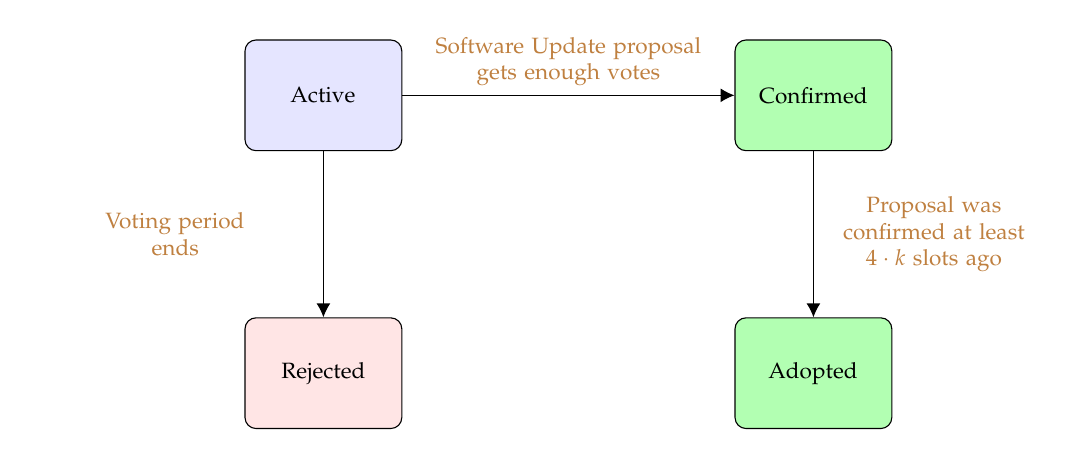
\begin{tikzpicture}[ align = center
                     , node distance = 6em and 12em
                     , text width = 5em
                     , font = \footnotesize
                     , >={Latex[width=0.5em, length=0.5em]}
                     , every node/.style = { rectangle
                                         , rounded corners
                                         , draw = black
                                         , align = center
                                         , minimum height = 4em }
                     ]

  \node (active) [fill = blue!10] {Active};
  \node (rejected) [below = of active, fill = red!10] {Rejected};
  \node (confirmed) [right = of active, fill = green!30] {Confirmed};
  \node (adopted) [below = of confirmed, fill = green!30] {Adopted};

  \tikzset{every node/.style={align=center, text width=10em, text=brown}}

  \draw[->] (active)
  edge node [above] {Software Update proposal\\ gets enough votes}
  (confirmed);

  \draw[->] (active)
  edge node [left] {Voting period \\ends}
  (rejected);

  \draw[->] (confirmed)
  edge node [right, text width=8em]
  {Proposal was confirmed at least $4 \cdot k$ slots ago}
  (adopted);


  \end{tikzpicture}

  \caption{State-transition diagram for software-updates}
  \label{fig:st-diagram-sw-up}
\end{figure}

\clearpage

A sequence of votes can be applied using $\trans{upivotes}{}$ transitions. The
inference rules for them are presented in \cref{fig:rules:apply-votes}. After
applying a sequence of votes, proposals might get confirmed, which means that
they will be added to the set $\var{cps'}$. In such case, the mapping of
application names to their latest version known to the ledger will be updated to
include the information about the confirmed proposals. Note that, unlike
protocol updates, software updates take effect as soon as a proposal is
confirmed (we cannot wait for stability since we need to preserve compatibility
with the existing chain, where there are software update proposals that were
adopted without waiting for $2\cdot k$ slots). In this rule, we also delete the
confirmed id's from the set of registered application update proposals
($\var{raus}$), since this information is no longer needed once the
application-name to software-version map ($\var{avs}$) is updated.

Also note that, unlike the rules of \cref{fig:rules:upi-ec}, we need not remove
other update proposals that refer to the software names whose versions were
changed in $\var{avs_{new}}$. The reason for this is that the range of $\var{raus}$
can contain only one pair of the form $(\var{an}, \wcard, \wcard)$ for any given
application name $\var{an}$ (see Rule~\ref{eq:rule:up-av-validity}).


\begin{figure}[htb]
  \begin{equation}
    \label{eq:rule:apply-votes-base}
    \inference
    {
    }
    {
      {\left(
        \begin{array}{l}
          s_n\\
          \var{dms}
        \end{array}
      \right)}
      \vdash
      \var{us}
      \trans{applyvotes}{\epsilon}
      \var{us}
    }
  \end{equation}
  %
  \nextdef
  %
  \begin{equation}
    \label{eq:rule:apply-votes-ind}
    \inference
    {
      {\left(
        \begin{array}{l}
          s_n\\
          \var{dms}
        \end{array}
      \right)}
      \vdash
      \var{us}
      \trans{applyvotes}{\Gamma}
      \var{us'}
      &
      {\left(
        \begin{array}{l}
          s_n\\
          \var{dms}
        \end{array}
      \right)}
      \vdash
      \var{us'}
      \trans{\hyperref[fig:rules:upi-vote]{upivote}}{v}
      \var{us''}
    }
    {
      {\left(
        \begin{array}{l}
          s_n\\
          \var{dms}
        \end{array}
      \right)}
      \vdash
      \var{us}
      \trans{applyvotes}{\Gamma;v}
      \var{us''}
    }
  \end{equation}
  %
  \nextdef
  %
  \begin{equation}
    \label{eq:rule:upivotes}
    \inference{
      {\left(
        \begin{array}{l}
          s_n\\
          \var{dms}
        \end{array}
      \right)}
      \vdash
      {\left(
          \begin{array}{l}
            (\var{pv}, \var{pps})\\
            \var{fads}\\
            \var{avs}\\
            \var{rpus}\\
            \var{raus}\\
            \var{cps}\\
            \var{vts}\\
            \var{bvs}\\
            \var{pws}
          \end{array}
        \right)}
      \trans{applyvotes}{\Gamma}
      {\left(
          \begin{array}{l}
            (\var{pv'}, \var{pps'})\\
            \var{fads'}\\
            \var{avs'}\\
            \var{rpus'}\\
            \var{raus'}\\
            \var{cps'}\\
            \var{vts'}\\
            \var{bvs'}\\
            \var{pws'}
          \end{array}
      \right)}\\
      %
      {\begin{array}{r@{~\leteq~}l}
        \var{cfm_{raus}} & \dom~(cps') \restrictdom \var{raus'}\\
        \var{avs_{new}} & \{ \var{an} \mapsto (\var{av}, \var{s_n}, m)
        \mid (\var{an}, \var{av}, m) \in \var{cfm_{raus}} \}
      \end{array}}
    }{
      {\left(
        \begin{array}{l}
          s_n\\
          \var{dms}
        \end{array}
      \right)}
      \vdash
      {\left(
          \begin{array}{l}
            (\var{pv}, \var{pps})\\
            \var{fads}\\
            \var{avs}\\
            \var{rpus}\\
            \var{raus}\\
            \var{cps}\\
            \var{vts}\\
            \var{bvs}\\
            \var{pws}
          \end{array}
      \right)}
      \trans{upivotes}{\Gamma}
      {\left(
          \begin{array}{l}
            (\var{pv'}, \var{pps'})\\
            \var{fads'}\\
            \var{avs'} \unionoverrideRight \var{avs_{new}}\\
            \var{rpus'}\\
            \dom~(cps') \subtractdom \var{raus'}\\
            \var{cps'}\\
            \var{vts'}\\
            \var{bvs'}\\
            \var{pws'}
          \end{array}
      \right)}
    }
  \end{equation}
  \caption{Applying multiple votes on update-proposals rules}
  \label{fig:rules:apply-votes}
\end{figure}
\clearpage

The interface rule for protocol-version endorsement makes use of the
$\trans{upend}{}$ transition, where we set the threshold for proposal adoption
to: the number of genesis keys ($\var{ngk}$) times the minimum proportion of
genesis keys that need to endorse an update proposal for it to become a
candidate for adoption (given by the protocol parameter $\var{upAdptThd}$). In
addition, the unconfirmed proposals that are older than $u$ blocks are removed
from the parts of the state that hold:
\begin{itemize}
\item the registered protocol and software update proposals,
\item the votes associated with the proposals,
\item the set of endorsement-key pairs, and
\item the block number in which proposals where added.
\end{itemize}

In Rule~\ref{eq:rule:upi-pend}, the set of proposal id's $\var{pid_{keep}}$
contains only those proposals that haven't expired yet or that are confirmed.
Once a proposal $\var{up}$ is confirmed, it is removed from the set of
confirmed proposals ($\var{cps}$) when a new a protocol version gets adopted
(see Rule~\ref{eq:rule:upi-ec-pv-change}).
%
The set of endorsement-key pairs is cleaned here as well as in the epoch change
rule (Rule~\ref{eq:rule:upi-ec-pv-change}). The reason for this is that this set grows at
each block, and it can get considerably large if no proposal gets adopted at
the end of an epoch.

\begin{figure}[htb]
  \begin{equation}
    \label{eq:rule:upi-pend}
    \inference
    {
      \var{upAdptThd} \mapsto q \in \var{pps} \\
      \left({
        \begin{array}{l}
          s_n\\
          \floor{q \cdot \var{ngk}}\\
          \var{dms}\\
          \var{cps}\\
          \var{rpus}
        \end{array}
      }\right)
      \vdash
      {
        \left(
          \begin{array}{l}
            \var{fads}\\
            \var{bvs}
          \end{array}
        \right)
      }
      \trans{\hyperref[fig:rules:up-end]{upend}}{(\var{bv}, \var{vk})}
      {
        \left(
          \begin{array}{l}
            \var{fads'}\\
            \var{bvs'}
          \end{array}
        \right)
      }\\
      \var{upropTTL} \mapsto u \in \var{pps}\\
      {
        \begin{array}{r@{~\leteq~}l}
          \var{pids_{keep}} & \dom~(pws \restrictrange [s_n - u, ..]) \cup \dom~\var{cps}\\
          \var{vs_{keep}} & \dom~(\range~\var{rpus'})\\
          \var{rpus'} & \var{pids_{keep}} \restrictdom \var{rpus}
        \end{array}
      }
    }
    {
      {\left(
        \begin{array}{l}
          s_n\\
          \var{dms}
        \end{array}
      \right)}
      \vdash
      {
        \left(
          \begin{array}{l}
            (\var{pv}, \var{pps})\\
            \var{fads}\\
            \var{avs}\\
            \var{rpus}\\
            \var{raus}\\
            \var{cps}\\
            \var{vts}\\
            \var{bvs}\\
            \var{pws}
          \end{array}
        \right)
      }
      \trans{upiend}{(\var{bv}, \var{vk})}
      {
        \left(
          \begin{array}{l}
            (\var{pv}, \var{pps})\\
            \var{fads'}\\
            \var{avs}\\
            \var{rpus'}\\
            \var{pids_{keep}} \restrictdom \var{raus}\\
            \var{cps}\\
            \var{pids_{keep}} \restrictdom \var{vts}\\
            \var{vs_{keep}}  \restrictdom \var{bvs'}\\
            \var{pids_{keep}} \restrictdom \var{pws}
          \end{array}
        \right)
      }
    }
  \end{equation}
  \caption{Proposal endorsement rules}
  \label{fig:rules:upi-pend}
\end{figure}

\clearpage

Rule~\ref{eq:rule:upi-ec-pv-change} models how the protocol-version and its
parameters are changed depending on an epoch change signal.
%
On an epoch change, this rule will pick a candidate that gathered enough
endorsements at least $4 \cdot k$ slots ago. If a protocol-version candidate
cannot gather enough endorsements $4 \cdot k$ slots before the end of an epoch,
the proposal can only be adopted in the next epoch. The reason for the $4 \cdot
k$ slot delay is to allow a period between knowing when a proposal will be
adopted, and the event of its being adopted. Since update proposals can and will
make large changes to the way the chain operates, it is useful to be able to
guarantee a window in which it is known that no update will take place.
%
Figure~\ref{fig:up-confirmed-too-late} shows an example of a proposal being
confirmed too late in an epoch, where it is not possible to get enough
endorsements in the remaining window. In this Figure we take $k = 2$, and we
assume $4$ endorsements are needed to consider a proposal as candidate for
adoption.
%
Note that, in the final state, we use union override to define the updated
parameters ($\var{pps} \unionoverrideRight \var{pps'}$). This is because candidate
proposal might only update some parameters of the protocol.

In Rule~\ref{eq:rule:upi-ec-pv-change}, when a new proposal gets adopted, all
the state components that refer to protocol update proposals get emptied. The
reason for this is that at the moment of registering a proposal, we evaluated
it in a state where the protocol parameters that we used for this are no longer
up to date (see for instance \cref{eq:func:can-update}). For instance, assume
we register a proposal $\var{up}$ which only changes the maximum transaction
size to $x$, and the current block size is set to $x + 1$. Then,
$\fun{canUpdate}$ holds, since the maximum transaction size is less than the
maximum block size. If now a new proposal gets adopted that changes the maximum
block size to $x - 1$, then this invalidates $\var{up}$ since $\fun{canUpdate}$
no longer holds.
%

If there are no candidates for adoption, then the state variables remain
unaltered (Rule~\ref{eq:rule:upi-ec-pv-unchanged}).

Also note that the registered software-update proposals need not be cleaned
here, since this is done either when a proposal gets confirmed or when it
expires.

\begin{figure}[htb]
  \begin{equation}
    \label{eq:rule:pvbump-change-epoch-only}
    \inference
    {
      [.., s_n - 4 \cdot k] \restrictdom \var{fads} = \epsilon
    }
    {
      {\left(\begin{array}{l}
         s_n\\
         \var{fads}
       \end{array}\right)}
      \vdash
      {
        \left(
          \begin{array}{l}
            \var{pv}, \var{pps}\\
          \end{array}
        \right)
      }
      \trans{pvbump}{}
      {
        \left(
          \begin{array}{l}
            \var{pv}, \var{pps}\\
          \end{array}
        \right)
      }
    }
  \end{equation}
  \nextdef
  \begin{equation}
    \label{eq:rule:pvbump-change}
    \inference
    {
      \wcard ; (\wcard , (\var{pv_c}, \var{pps_c})) \leteq [.., s_n - 4 \cdot k] \restrictdom \var{fads}
    }
    {
      {\left(\begin{array}{l}
         s_n\\
         \var{fads}
       \end{array}\right)}
      \vdash
      {
        \left(
          \begin{array}{l}
            \var{pv}, \var{pps}\\
          \end{array}
        \right)
      }
      \trans{pvbump}{}
      {
        \left(
          \begin{array}{l}
            \var{pv_c}, \var{pps_c}\\
          \end{array}
        \right)
      }
    }
  \end{equation}
  \caption{Protocol version bump rules}
  \label{fig:rules:pvbump}
\end{figure}

\begin{figure}[htb]
  \begin{equation}
    \label{eq:rule:upi-ec-pv-unchanged}
    \inference
    {
      {\left(\begin{array}{l}
         \fun{firstSlot}~e_n\\
         \var{fads}
       \end{array}\right)}
      \vdash
      {
        \left(
          \begin{array}{l}
            \var{pv}, \var{pps}
          \end{array}
        \right)
      }
      \trans{\hyperref[fig:rules:pvbump]{pvbump}}{}
      {
        \left(
          \begin{array}{l}
            \var{pv'}, \var{pps'}\\
          \end{array}
        \right)
      } &\var{pv} = \var{pv'}
    }
    {
      (e_n)
      \vdash
      {
        \left(
          \begin{array}{l}
            (\var{pv}, \var{pps})\\
            \var{fads}\\
            \var{avs}\\
            \var{rpus}\\
            \var{raus}\\
            \var{cps}\\
            \var{vts}\\
            \var{bvs}\\
            \var{pws}
          \end{array}
        \right)
      }
      \trans{upiec}{}
      {
        \left(
          \begin{array}{l}
            (\var{pv}, \var{pps})\\
            \var{fads}\\
            \var{avs}\\
            \var{rpus}\\
            \var{raus}\\
            \var{cps}\\
            \var{vts}\\
            \var{bvs}\\
            \var{pws}
          \end{array}
        \right)
      }
    }
  \end{equation}
  \nextdef
  \begin{equation}
    \label{eq:rule:upi-ec-pv-change}
    \inference
    {
      {\left(\begin{array}{l}
         \fun{firstSlot}~e_n\\
         \var{fads}
       \end{array}\right)}
      \vdash
      {
        \left(
          \begin{array}{l}
            \var{pv}, \var{pps}\\
          \end{array}
        \right)
      }
      \trans{\hyperref[fig:rules:pvbump]{pvbump}}{}
      {
        \left(
          \begin{array}{l}
            \var{pv'}, \var{pps'}\\
          \end{array}
        \right)
      }
      & \var{pv} \neq \var{pv'}
    }
    {
      (e_n)
      \vdash
      {
        \left(
          \begin{array}{l}
            \var{(\var{pv}, \var{pps})}\\
            \var{fads}\\
            \var{avs}\\
            \var{rpus}\\
            \var{raus}\\
            \var{cps}\\
            \var{vts}\\
            \var{bvs}\\
            \var{pws}
          \end{array}
        \right)
      }
      \trans{upiec}{}
      {
        \left(
          \begin{array}{l}
            (\var{pv'}, \var{pps'})\\
            \epsilon\\
            \var{avs}\\
            \emptyset\\
            \emptyset\\
            \emptyset\\
            \emptyset\\
            \emptyset\\
            \emptyset\\
          \end{array}
        \right)
      }
    }
  \end{equation}
  \caption{Block version adoption on epoch change rules}
  \label{fig:rules:upi-ec}
\end{figure}

\begin{figure}[htb]
  \centering
  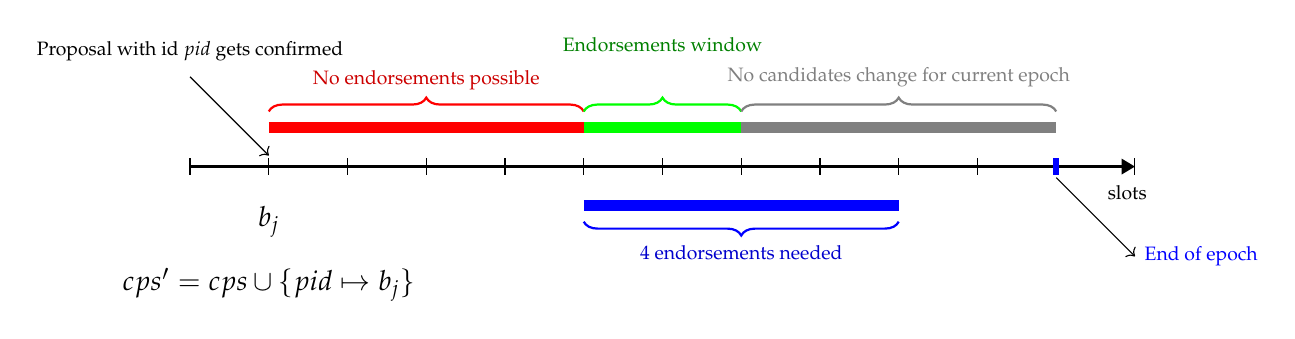
\begin{tikzpicture}
    %%
    %% Macros used in this picture
    %%
    %
    % Number of slots
    \pgfmathsetmacro{\nrSlots}{12}
    % Slot in which the proposal gets confirmed
    \pgfmathsetmacro{\cSlot}{1}
    % Our special K.
    \pgfmathsetmacro{\K}{4}
    % Epoch end.
    \pgfmathsetmacro{\eend}{11}
    % Number of positive votes needed
    \pgfmathsetmacro{\votes}{4}

    % Draw the horizontal line
    \draw[thick, -Triangle] (0,0) -- (\nrSlots,0)
    node[font=\scriptsize,below left=3pt and -8pt]{slots};

    % % draw vertical lines
    \foreach \x in {0,1,...,\nrSlots}
    \draw (\x cm, 3pt) -- (\x cm, -3pt);

    % Add a label to with the block number in which the proposal got confirmed.
    \node at (\cSlot, -.7) {$b_j$};

    % Update in cps
    \node at (\cSlot, -1.5) {$\var{cps'} = \var{cps} \cup \{ \var{pid} \mapsto b_j \}$};

    % The no-endorsements red bar.
    \draw[red, line width=4pt] (\cSlot, .5) -- +(\K, 0);

    % Brace above the no-endorsement window bar.
    \draw[thick, red, decorate, decoration={brace, amplitude=5pt}]
    (\cSlot, .7) -- +(\K, 0)
    node[black!20!red, midway, above=4pt, font=\scriptsize] {No endorsements possible};

    % The endorsements window.
    \coordinate (ewStart) at (\cSlot + \K, .5);
    \coordinate (ewEnd) at ($(\eend - \K, .5)$);
    \draw[green, line width=4pt]
    (ewStart) -- (ewEnd);

    % Brace above the endorsements window
    \coordinate (ewStartB) at ($(ewStart) + (0, 0.2)$);
    \coordinate (ewEndB) at ($(ewEnd) + (0, 0.2)$);
    \draw[thick, green, decorate, decoration={brace, amplitude=5pt}]
    (ewStartB) -- (ewEndB)
    node[black!50!green, midway, above=18pt, font=\scriptsize] {Endorsements window};

    % The no-candidates change window.
    \coordinate (nccStart) at (\eend - \K, .5);
    \coordinate (nccEnd) at ($(\eend, .5)$);
    \draw[gray, line width=4pt]
    (nccStart) -- (nccEnd);

    % Brace above the no-candidates change window.
    \coordinate (nccStartB) at ($(nccStart) + (0, 0.2)$);
    \coordinate (nccEndB) at ($(nccEnd) + (0, 0.2)$);
    \draw[thick, gray, decorate, decoration={brace, amplitude=5pt}]
    (nccStartB) -- (nccEndB)
    node[gray, midway, above=5pt, font=\scriptsize] {No candidates change for current epoch};


    % The 2k before end-of-epoch window.
    \coordinate (beeStart) at (\cSlot + \K, -.5);
    \coordinate (beeEnd) at ($(\cSlot + \K + \votes, -.5)$);
    \draw[blue, line width=4pt]
    (beeStart) -- (beeEnd);

    % Brace on above the 2k before end-of-epoch window.
    \coordinate (beeStartB) at ($(beeStart) - (0, 0.2)$);
    \coordinate (beeEndB) at ($(beeEnd) - (0, 0.2)$);
    \draw[thick, blue, decorate, decoration={brace, amplitude=5pt}]
    (beeEndB) -- (beeStartB)
    node[black!20!blue, midway, below=5pt, font=\scriptsize] {$\votes$ endorsements needed};

    \draw[blue, line width=2pt] (\eend, 3pt) -- (\eend, -3pt);

    \draw[<-] (\cSlot, 4pt) -- +(-1, 1)
    node [above=2pt, black, font=\scriptsize]
    {Proposal with id $\var{pid}$ gets confirmed};

    \draw[->] (\eend, -4pt) -- +(1, -1)
    node[right, blue, font=\scriptsize] {End of epoch};
  \end{tikzpicture}
  \caption{An update proposal confirmed too late}
  \label{fig:up-confirmed-too-late}
\end{figure}

Figure~\ref{fig:st-diagram-pt-up} shows the different states a protocol-update
proposal can be in, and what causes the transitions between them.

\begin{figure}[ht]
  \centering
  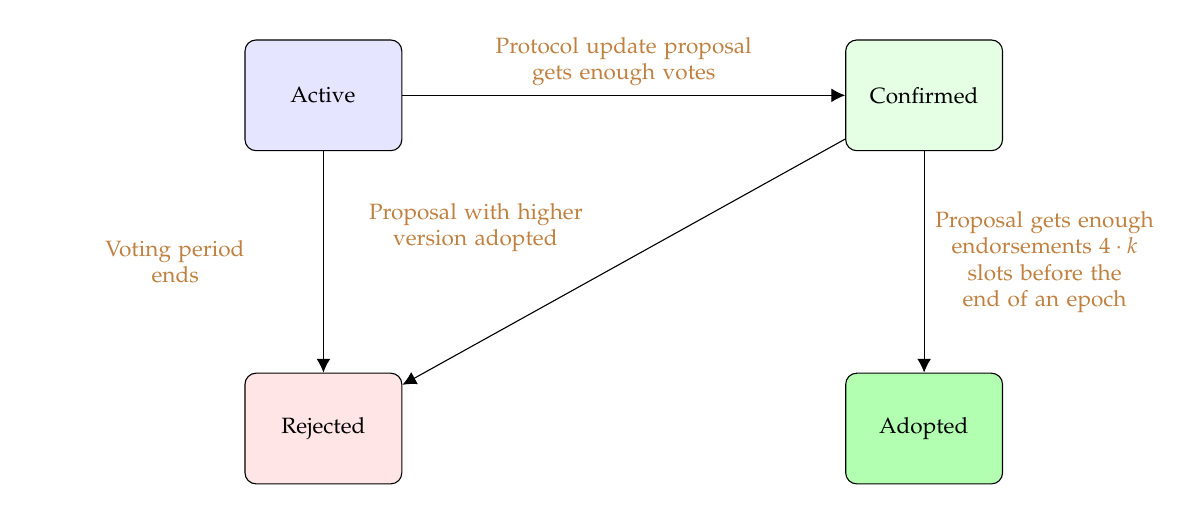
\begin{tikzpicture}[ align = center
                     , node distance = 8em and 16em
                     , text width = 5em
                     , font = \footnotesize
                     , >={Latex[width=0.5em, length=0.5em]}
                     , every node/.style = { rectangle
                                         , rounded corners
                                         , draw = black
                                         , align = center
                                         , minimum height = 4em }
                     ]

  \node (active) [fill = blue!10] {Active};
  \node (rejected) [below = of active, fill = red!10] {Rejected};
  \node (confirmed) [right = of active, fill = green!10] {Confirmed};
  \node (adopted) [below = of confirmed, fill = green!30] {Adopted};

  \tikzset{every node/.style={align=center, text width=10em, text=brown}}

  \draw[->] (active)
  edge node [above] {Protocol update proposal\\ gets enough votes}
  (confirmed);

  \draw[->] (active)
  edge node [left] {Voting period \\ends}
  (rejected);

  \draw[->] (confirmed)
  edge node [above left]
  {Proposal with higher version adopted}
  (rejected);

  \draw[->] (confirmed)
  edge node [right, text width=8em]
  {Proposal gets enough endorsements $4 \cdot k$ slots before the end of an epoch}
  (adopted);

  \end{tikzpicture}

  \caption{State-transition diagram for protocol-updates}
  \label{fig:st-diagram-pt-up}
\end{figure}


\section{Formal Properties}
\label{sec:properties}

This appendix collects the main formal properties that the new ledger rules are expected to satisfy.
Note here that in every property in this section we consider a only phase-1 valid
transactions, ie. ones that can indeed get processed.

\begin{enumerate}[label=P{\arabic*}:\ ]
\item
  \emph{Consistency with Shelley.}
  \begin{itemize}
    \item properties 15.6 - 15.16 (except 15.8 and 15.13) hold specifically in the $\fun{txValTag}~tx~=~\True$ case, because
    the calculations refer to the UTxO as if it was updated by a scripts-validating transaction
    \item other properties hold as-is
  \end{itemize}

\item
  \emph{Consistency with Multi-Asset.}
  \begin{itemize}
    \item properties 8.1 and 8.2 hold specifically in the $\fun{txValTag}~tx~=~\True$ case, because
    the calculations refer to the UTxO as if it was updated by a scripts-validating transaction
    \item other properties hold as-is
  \end{itemize}
\end{enumerate}


\begin{definition}
  For a state $s$ that is used in any subtransaction of
  $\mathsf{CHAIN}$, we define $\Utxo(s) \in \UTxO$ to be the $\UTxO$
  contained in $s$, or an empty map if it does not exist. This is
  similar to the definition of $\Val$ in the Shelley specification.

  Similarly, we also define $\field_{v}~(s)$ for the field $v$ that is part of
  the ledger state $s$, referenced by the typical variable name (eg. $\var{fees}$
  for the fee pot on the ledger).
\end{definition}

We also define a helper function $\varphi$ as follows:
\[\varphi(x, tx) :=
  \begin{cases}
    x & \fun{txValTag}~tx = \True \\
    0 & \fun{txValTag}~tx = \False
  \end{cases}\]
This function is useful to distinguish between the two
cases where a transaction can mint tokens or not, depending on whether
its scripts validate.

\begin{property}[General Accounting]
  \label{prop:pov}
  The \emph{general accounting} property in Alonzo encompasses two parts
  \begin{itemize}
    \item preservation of value property expressed via the $\fun{produced}$ and $\fun{consumed}$
    calculations, applicable for transactions with $\fun{txValTag}~tx~=~\True$, which
    is specified as in the ShelleyMA POV.
    \item the preservation of value for $\fun{txValTag}~tx~=~\False$, when
    only the collateral fees are collected into the fee pot.
  \end{itemize}

Both of these are expressed in the following lemma.

\begin{lemma}
  For all environments $e$, transactions $tx$ and states $s, s'$, if
  \begin{equation*}
    e\vdash s\trans{utxos}{tx}s'
  \end{equation*}
  then
  \begin{equation*}
    \Val(s) + \varphi(\fun{mint}~(\fun{txbody}~tx), tx) = \Val(s')
  \end{equation*}
\end{lemma}

\begin{proof}
  In the case that $\fun{txValTag}~tx = \True$ holds, the proof is
  identical to the proof of Lemma 9.1 of the multi-asset
  specification. Otherwise, the transition must have been done via the
  $\mathsf{Scripts-No}$ rule, which removes
  $\fun{collateral}~(\fun{txbody}~tx)$ from the UTxO, and increases the fee pot by the amount of the sum of Ada in the
  collateral UTxO entries. The value contained in $s$ is not changed.

  Note that in the $\fun{feesOK}$ function, there is a check that verifies
  that, in the case that there are phase-2 scripts, there are no non-Ada tokens in the UTxOs
  which the collateral inputs reference, so non-Ada tokens do not get minted, burned, or transferred
  in this case.
\end{proof}
\end{property}

\begin{property}[Extended UTxO Validation]
  \label{prop:fees-only}

  If a phase-1 valid transaction extends the UTxO, all its scripts validate
  (i.e. $\fun{txValTag}~tx = \True$).

  If a transaction is accepted and marked as paying collateral only
  (i.e. $\fun{txValTag}~tx = \False$), then the only change to the ledger
  when processing the transaction is that the collateral inputs
  are moved to the fee pot. In particular, it does not extend the UTxO.

  \begin{lemma}
    For all environments $e$, transactions $tx$ and states $s, s'$, if  and
    \begin{equation*}
      e\vdash s\trans{ledger}{tx}s'
    \end{equation*}
    then
    \[\Utxo(s') \nsubseteq \Utxo(s)~\Rightarrow~\fun{txValTag}~tx = \True \]

    Also,
    \[\fun{txvaltag}~tx = \False~ \Rightarrow~\]
    \begin{itemize}
      \item $ \field_{v}~(s') = \field_{v}~(s) \text{ for all } v~\neq~{fees}, ~v~\neq~{utxo}$
      \item $\field_{fees}~(s') = \field~\var{fees}~(s) + \fun{coin}~(\Val~(\fun{collateral}~{tx} \subtractdom \Utxo(s)))$
      \item $\Utxo(s') = \fun{collateral}~{tx} \subtractdom \Utxo(s)$
    \end{itemize}
  \end{lemma}

  \begin{proof}
    A ledger UTxO update is specified explicitly only by the $\mathsf{UTXOS}$ transition,
    and propagated (ie. applied as-specified) to a chain-state update via the
    $\mathsf{UTXO}$ and $\mathsf{UTXOW}$ transitions.

    The only case in which the $\mathsf{UTXOS}$ transition adds entries to the UTxO
    map is in the $\mathsf{Scripts-No}$ rule, when $\fun{txValTag}~tx = \True$.
    Adding entries to the UTxO map implies exactly that the updated map is not a
    submap of the original, so we get that

    \[\Utxo(s') \nsubseteq \Utxo(s)~\Rightarrow~\fun{txValTag}~tx = \True \]

   In the case that $\fun{txValTag}~tx = \False$, $\mathsf{LEDGER}$ calls the rule
   that does not update $\DPState$ at all, only the $\UTxOState$. This state update is specified
   in the $\mathsf{UTXOS}$ transition (and applied via the $\mathsf{UTXO}$ and $\mathsf{UTXOW}$ transitions).

   The only parts of the state that are updated are
   \begin{itemize}
     \item the fee pot, which is increased by the amount of the sum of Ada in the
     collateral UTxO entries, and
     \item the UTxO, where the collateral entries
     are removed.
   \end{itemize}
  \end{proof}
\end {property}

\begin{property}[Validating when No NN Scripts]
  \label{prop:is-valid}

Whenever a valid transaction does not have any phase-2 scripts, its
$\fun{txValTag} = \True$.

\begin{lemma}
  For all environments $e$, transactions $tx$ and states $s, s'$ such that
  \begin{equation*}
    e\vdash s\trans{ledger}{tx}s',
  \end{equation*}
  If $\range (\fun{txscripts}~tx) \cap \ScriptPhTwo = \emptyset$
  then $\fun{txValTag} = \True$.
\end{lemma}
\begin{proof}
  With the same argument as previously, we only need to discuss the
  equivalent claim for the $\mathsf{UTXOS}$ transition. Under these
  assumptions, $\var{sLst}$ is an empty
  list. Thus $\fun{evalScripts}~sLst = \True$, and the transition rule
  had to be $\mathsf{Scripts{-}Yes}$.
\end{proof}
\end{property}

\begin{property}[Paying fees]
  \label{prop:pay-fees}

In the case that all phase-2 scripts in a transaction validate, the transaction pays
at least the minimum transaction fee amount into the fee pot. In the case that
some do not validate, it must pay at least the percentage of the minimum fee
the collateral is required to cover.

\begin{lemma}
  For all environments $e$, transactions $tx$ and states $s, s'$ such that
  \begin{equation*}
    e\vdash s\trans{ledger}{tx}s'
  \end{equation*}
  The following holds : \\
  $\field_{fees}~(s')~\geq~\field_{fees}~(s)~+
  \begin{cases}
    \fun{minfee}~{tx} & \fun{txValTag} = \True \\
    \fun{quot}~(\fun{collateralPercent}~(\field_{pp}~(s)))~*~(\fun{minfee}~{tx})~100 & \fun{txValTag} = \False\\
  \end{cases}$.
\end{lemma}
\begin{proof}
  The fee pot is updated by the $\mathsf{Scripts{-}Yes}$ and the $\mathsf{Scripts{-}No}$
  rules, one of which is necessarily called by a valid transaction via the sequence
  of transitions called in the order $\mathsf{LEDGER}, \mathsf{UTXOW}, \mathsf{UTXO}, \mathsf{UTXOS}$.

  The $\mathsf{Scripts{-}Yes}$ rule (i.e. $\fun{txValTag} = \True$)
  transfers the amount of Lovelace in the $\fun{txfee}$ field of the
  transaction to the fee pot, which is checked to be at least the $\fun{minfee}$
  by $\fun{feesOK}$ in the $\mathsf{UTXO}$ transition. So, we get

  \[\field_{fees}~(s')~=~\field_{fees}~(s)~+~\fun{txfee}~{tx}~\geq~\field_{fees}~(s)~+~\fun{minfee}~{tx}\]

  The $\mathsf{Scripts{-}No}$ rule (i.e. $\fun{txValTag} = \False$) removes the
  $\fun{collateral}$ inputs from the
  UTxO, and adds the balance of these realized inputs to the fee pot.

  \[\field_{fees}~(s')~=~field_{fees}~(s)~+~\fun{ubalance}~(\fun{collateral}~{txb} \restrictdom \var{utxo})\]

  We can conclude that $\fun{txrdmrs}$ is non-empty whenever $\fun{txValTag} = \False$
  from the following observations :
  \begin{itemize}
    \item $\fun{txValTag} = \False$ whenever $\fun{evalScripts}$ fails.
    \item $\fun{evalScripts}$ is a $\wedge$-fold over a list of scripts and
    their inputs, containing all scripts that need to be run to validate this transaction
    \item All phase-1 scripts must succeed, as this is checked in phase-1 validation (UTXOW
    rule check). Therefore,
    $\fun{evalScripts}$ encounters a failing script which is phase-2.
    \item All phase-2 scripts necessarily have an associated redeemer attached to the
    transaction (UTXOW rule check)
  \end{itemize}

  See Property~\ref{prop:fixed-inputs} for more details on what inputs $\fun{evalScripts}$ has,
  and what we can say about the outcome of its computation with respect to its inputs.

  The $\fun{feesOK}$ check enforces that if a transaction has a non-empty
  $\fun{txrdmrs}$ field, the balance of the realized collateral inputs
  (which $\field_{fees}~(s)$ is increased by as part of processing $tx$) is

  \[\fun{ubalance}~(\fun{collateral}~{txb} \restrictdom \var{utxo})~\geq~\fun{quot}~(\txfee~{txb} * (\fun{collateralPercent}~pp))~100\]

  which, since $\txfee~{txb}~\geq~\fun{minfee}~{txb}$, gives

  \[ \geq~\fun{quot}~(\fun{minfee}~{txb} * (\fun{collateralPercent}~pp))~100)) \]

  where $\fun{txbody}~{tx}~=~{txb}$. This shows that the total collateral that gets
  moved into the fee pot from the UTxO by the $\mathsf{Scripts{-}No}$ rule is at
  least the minimum transaction fee scaled by the collateral percent parameter.

  \[\field_{fees}~(s')~\geq~\field_{fees}~(s)~+~\fun{quot}~(\fun{minfee}~{txb} * (\fun{collateralPercent}~pp))~100))\]
\end{proof}

An immediate corollary to this property is that when the $\fun{collateralPercent}$ is set to 100 or more,
the transaction always pays at least the minimum fee. This, in turn, implies that it
pays at least the fee that it has stated in the $\fun{txfee}$ field.

\begin{corollary}
  For all environments $e$, transactions $tx$ and states $s, s'$ such that
  \begin{equation*}
    e\vdash s\trans{ledger}{tx}s'~~\wedge~~\fun{collateralPercent}~(\field_{pp}~(s)) \geq 100
  \end{equation*}
  The following holds :
  \[\field_{fees}~(s')~\geq~\field_{fees}~(s)~+~\fun{minfee}~{tx} \]
\end{corollary}

\begin{proof}
  In both two cases in the lemma above, the $\field_{fees}$ field in the ledger state
  is increased by at least $\fun{minfee}~{tx}$ :
  \begin{itemize}
    \item when $\fun{txValTag} = \True$, the lemma states already that
    \[\field_{fees}~(s')~\geq~\field_{fees}~(s)~+~\fun{minfee}~{tx}\]
    \item when $\fun{txValTag} = \False$, we have
    $ \field_{fees}~(s')~\geq~\field_{fees}~(s)~+~\fun{quot}~(\fun{minfee}~{txb} * (\fun{collateralPercent}~pp))~100$ \\
    $~~~\geq~\field_{fees}~(s)~+~\fun{quot}~(\fun{minfee}~{tx}~*~100)~100$ \\
    $~~~=~\field_{fees}~(s)~+~\fun{minfee}~{tx}$
  \end{itemize}
\end{proof}

\end{property}

\begin{property}[Correct tag]
  \label{prop:correct-tag}

The $\fun{txValTag}~tx$ tag of a phase-1 valid transaction must match the result of the $\fun{evalScripts}$
function for that transaction.

\begin{lemma}
  For all environments $e$, transactions $tx$ and states $s, s'$ such that
  \begin{equation*}
    e\vdash s\trans{utxos}{tx}s',
  \end{equation*}
  The following holds :
    \[\fun{txValTag}~tx ~=~ \fun{evalScripts}~{tx}~{sLst} \]
  where
  \[ \var{sLst} \leteq \fun{collectTwoPhaseScriptInputs}~\mathsf{EI}~\mathsf{SysSt} ~\field_{pp}(s)~\var{tx}~ \Utxo(s) \]
\end{lemma}
\begin{proof}
  Inspecting the $\mathsf{Scripts{-}Yes}$ and the $\mathsf{Scripts{-}No}$ rules of the $\mathsf{UTXOS}$ transition,
  we see that both the $\fun{txValTag}$ and the result of $\fun{evalScripts}$
  are $\True$ in the former, and $\False$ in the latter.
\end{proof}
\end{property}

\begin{property}[Replay protection]
  \label{prop:replay}

A transaction always removes at least one UTxO entry from the ledger, which provides
replay protection.

\begin{lemma}
  For all environments $e$, transactions $tx$ and states $s, s'$ such that
  \begin{equation*}
    e\vdash s\trans{ledger}{tx}s',
  \end{equation*}
  The following holds : $\Utxo~(s)~\nsubseteq~\Utxo~(s')$.
\end{lemma}
\begin{proof}
  The UTxO is updated by the $\mathsf{Scripts{-}Yes}$ and the $\mathsf{Scripts{-}No}$
  rules, on of which is necessarily called by a valid transaction. Both of these
  rules remove UTxOs corresponding to a set of inputs.

  In both cases, there is a check that the removed inputs set is non-empty.
  The $\mathsf{Scripts{-}Yes}$ rule of the $\mathsf{UTXOS}$ transition
  removes the UTxOs associated with the input set $\fun{txinputs}~{tx}$ from the ledger.
  The $\fun{txinputs}~{tx}$ set must be non-empty because there is a check in the
  $\mathsf{UTXO}$ rule (which calls $\mathsf{UTXOS}$) that ensure this is true.

  For the $\mathsf{Scripts{-}No}$ rule of the $\mathsf{UTXOS}$ transition
  removes the UTxOs associated with the input set $\fun{collateral}~{tx}$ from the ledger.
  The $\fun{collateral}~{tx}$ set must be non-empty because
  the $\fun{feesOK}$ function (called by the same rule that calls $\mathsf{UTXO},
  \mathsf{UTXOS}$) ensures that in the case that the $tx$ contains phase-2 scripts,
  $\fun{collateral}~{tx}$ must be non-empty.

  Note that by property~\ref{prop:is-valid}, phase-2 scripts must always be present
  if $\fun{txValTag}~tx = \False$ (that is, whenever $\mathsf{Scripts{-}No}$ rule is used).
\end{proof}
\end{property}

\begin{property}[UTxO-changing transitions]
  \label{prop:utxo-change}

The $\mathsf{UTXOS}$ transition fully specifies the change in the ledger $\UTxO$
for each transaction.

\begin{lemma}
  For all environments $e$, transitions $\mathsf{TRNS}$, transactions $tx$ and states $s, s'$ such that
  \begin{equation*}
    e\vdash s\trans{trns}{tx}s'
  \end{equation*}
  The following holds :
  \begin{equation*}
    \Utxo(s) \neq \Utxo(s')~\Rightarrow~e'\vdash u\trans{utxos}{tx}u'
  \end{equation*}
  where $\Utxo(s) = \Utxo(u)~\wedge~\Utxo(s') = \Utxo(u')$ for some environment $e'$,
  and states $u, u'$.
\end{lemma}
\begin{proof}
  By inspecting each transition in this specification, as well as those inherited from the
    Shelley one, we see that a non-trivial update from the UTxO of $s$ to that of $s'$
    must be done by $\mathsf{UTXOS}$. Every other transition that changes the UTxO and
    has a signal of type $\Tx$ only applies the $\mathsf{UTXOS}$.
\end{proof}
\end{property}

\begin{property}[Deterministic script evaluation]
  \label{prop:fixed-inputs}

The deterministic script evaluation property, also stated as
"script interpreter arguments are fixed", is a property of the Alonzo ledger
that guarantees that the outcome of phase-2 script validation in a (phase-1 valid) transaction
depends only on the contents of that transaction, and not on when, by who, or in what
block that transaction was submitted.

For this property, we make some assumptions about things that are outside the scope of this specification :

\begin{itemize}
  \item The Plutus script
  interpreter is a pure function that receives only the arguments provided by the ledger when it is
  invoked by calling the $\fun{runPLCScript}$ function. We assume that this is
  also true in an implementation. In particular, the interpreter does not
  obtain any system randomness, etc.

  \item We do not need to check here that the hashes that are the keys of the
  $\fun{txscripts}$ and $\fun{txdats}$ fields match the computed hashes of the scripts and
  datum objects they index. This is because these hashes must be computed as part of
  the deserialization of a transaction (see the CDDL specification),
  instead of being transmitted as part of the transaction and then checked. We
  assume these hashes are correct.

  \item We assume that the consensus
  function $\fun{epochInfoSlotToUTCTime}$ for converting a slot interval into a
  system time interval is deterministic.

  \item We assume that the two global
  constants, $\EpochInfo$ and $\SystemStart$, which it also takes as parameters,
  cannot change within the span of any interval for which $\fun{epochInfoSlotToUTCTime}$
  is able to convert both endpoints to system time.
\end{itemize}

The assumptions above are implicit in the functional style of definitions in this
specification, but they are worth pointing out for implementation.
With these assumptions in mind, we can say that
script evaluation is deterministic.

We split this result into a lemma and its corollary :

\begin{itemize}
  \item First, we demonstrate that all the scripts and their arguments that are
  collected for phase-2 validation are the same for two phase-1 valid transactions with the same body,
  independent of the (necessarily valid) ledger state to which they are being applied

  \item Second, we derive the corollary that under the same validity assumptions,
  phase-2 validation results in the same outcome for both transactions
\end{itemize}

\begin{lemma}
  \label{lem:inputs}
  For all environments $e, e'$, transactions $tx, tx'$ and states $s, s', u, u'$ such that
  $e$ and $s$ are subsets of fields of some valid chain state $c$, and
  $e'$ and $s'$ are subsets of fields of some valid chain state $c'$,

  \begin{equation*}
    e\vdash s\trans{ledger}{tx}s', \\
    e'\vdash u\trans{ledger}{tx'}u', \\
    \txbody{tx} = \txbody{tx'}
  \end{equation*}

  The following holds :

  \[\fun{toSet}~(\fun{collectTwoPhaseScriptInputs}~\mathsf{EI}~\mathsf{SysSt} ~\field_{pp}(s)~\var{tx}~ \Utxo(s))\]
  \[ = \]
  \[\fun{toSet}~(\fun{collectTwoPhaseScriptInputs}~\mathsf{EI}~\mathsf{SysSt} ~\field_{pp}(u)~\var{tx'}~ \Utxo(u))\]

\end{lemma}
\begin{proof}

    The $\fun{collectTwoPhaseScriptInputs}$
    function (see \ref{fig:functions:script2})
    constructs a list where each entry contains a Plutus script
    and the arguments passed to the interpreter for its evaluation.

    To show that $\fun{collectTwoPhaseScriptInputs}$ returns a list containing
    the same elements for both $tx$ and $tx'$, we observe that
    the set of elements from which this list is produced via $\fun{toList}$
    is generated using the following functions, as well as set comprehension
    and list operations.
    We demonstrate that the functions used in this definition
    produce the same output for $tx$ and $tx'$, as all the data they
    inspect is fixed by the transaction body :

    \begin{itemize}
      \item $\fun{scriptsNeeded}$ : The $\PolicyID$, $\AddrRWD$, and $\DCert$ data
      output by this function as the second term of the hash-purpose pair
      is obtained directly from the $\fun{mint}$, $\fun{txwdrls}$,
      $\fun{txcerts}$ fields of the transaction, which are all fixed by the
      body of the transaction. These types of script purposes all include
      the hash of the validating script.

      The only other data this function inspects is the UTxO entries associated
      with the $\fun{txinputs}$ (passed via the $\UTxO$ argument) to get the realized inputs.
      We know that the UTxO is a field in a valid chain state for both the phase-1 valid
      transactions $tx$ and
      the $tx'$ ($\Utxo(s)$ and $\Utxo(u)$, respectively). This means that the $\TxId$
      in each input present in either UTxO is a hash of the body of the transaction
      containing the $\TxOut$ part of the UTxO entry indexed by that input. The
      order of the outputs is also fixed by the body, which fixes the $\Ix$ of
      the entry.

      A different value in output part of the UTxO entry (or a different order of
      outputs) would necessarily imply
      that the hash of the body containing that output must be different.
      Therefore, for all Plutus script-locked realized inputs of either transaction,
      the script hash in the payment credential of the address
      (and, by the same argument, the datum hash) are fixed by the inputs in body of the
      transaction, despite not being explicitly contained in it. We then get that

      \[ \fun{scriptsNeeded}~\Utxo(s)~(\txbody{tx}) = \fun{scriptsNeeded}~\Utxo(u)~(\txbody{tx'}) \]

      \item $\fun{getDatum}$ : In the case the script purpose
      is of the input type, the datum this function returns is one that
      is associated with the corresponding realized input. More precisely, it is the datum whose
      hash is specified in the realized input, and is looked up by hash in the $\fun{txdats}$
      transaction field. If there is no datum hash in the realized input, or the script purpose
      is of a non-input type, the empty list is returned.

      The $\mathsf{UTXOW}$ rule checks that the transaction is carrying all datums corresponding
      to its realized inputs. Since the inputs (and realized inputs) are the same
      for $tx$ and $tx'$ (fixed by the body), this guarantees that
      of the datum hashes in the realized inputs (and therefore, their preimages)
      are the same as well.

      \item $\fun{txscripts}$ : in the $\mathsf{UTXOW}$ rule, there is a check that all the
      script preimages of the script hashes returned by the $\fun{scriptsNeeded}$
      function must be present in this field.

      \item $\fun{indexedRdmrs}$ : like $\fun{scriptsNeeded}$, this function
      examines four fields fixed by the transaction body ($\fun{mint}$, $\fun{txwdrls}$,
      $\fun{txcerts}$, and $\fun{txinputs}$).
      It also looks at data in the $\fun{txrdmrs}$ field, which is fixed
      by the transaction body via the $\fun{scriptIntegrityHash}$
      hash. This is done as follows: the $\mathsf{UTXOW}$ rule verifies that this
      hash-containing field matches the computed hash
      of the preimage constructed from several fields of the transaction,
      including $\fun{txrdmrs}$ (this calculation
      is done by the $\fun{hashScriptIntegrity}$ function).

      \item $\fun{language}$ : this is directly conveyed by the type of a script.

      \item $\fun{costmdls}$ : The hash calculated by the $\fun{hashScriptIntegrity}$
      function and compared to the hash value in the $\fun{scriptIntegrityHash}$ field
      must include in the preimage the current cost models of
      all script languages of scripts carried by the transaction. Recall that
      if a cost model changed between when a transaction was submitted and the
      time at which it was processed, the field and the calculated hash values
      will not match.

      \item $\fun{valContext}$ and $\fun{txInfo}$ :
      The $\fun{valContext}$ function is defined in \ref{sec:txinfo} and is pure.
      All fields of the $\TxInfo$
      structure, with the exceptions listed below,
      are straightforward translations of the corresponding transaction body fields (see \ref{sec:txinfo}) that
      are given no additional arguments,
      and therefore completely determined by $tx$ and $tx'$. The fields not directly
      appearing in the body are :

      \begin{itemize}
        \item $\fun{txInfoInputs}$ : this field contains the realized inputs of
        the transaction which are fixed by the transaction and the unique
        UTxO entries to which the inputs correspond. As explained above,
        accessing information in realized inputs for script evaluation
        does not break determinism.

        \item $\fun{txInfoValidRange}$ : this field contains the transaction
        validity interval as system time (converted from the slot numbers, which are
        used to specify the interval in the transaction body). This conversion is
        done by a function defined in the consensus layer, and takes two global
        constants in addition to the slot interval itself. Since the slot interval
        conversion function $\fun{epochInfoSlotToUTCTime}$ necessarily
        succeeds if both $tx$ and $tx'$ pass phase-1 validation, the additional
        global constant arguments must be the same (by assumption). The determinism of this conversion
        is one of the assumptions of this property, and thus gives the same output
        for both transactions.

        \item $\fun{txInfoData}$ : this field is populated with the datums (and their
        hashes) in the transaction field $\fun{txdats}$, which are fixed by the body
        via the $\fun{scriptIntegrityHash}$ field.

        \item $\fun{txInfoId}$ : this field contains the hash of the transaction body,
        which is clearly the same for transactions with the same body.
      \end{itemize}

      Therefore, each field of the $\TxInfo$ structure is
      the same for two transactions with the same body, ie.

      \[ \fun{txInfo}~\PlutusVI~\Utxo(s)~\var{tx} = \fun{txInfo}~\PlutusVI~\Utxo(u)~\var{tx'}\]

    \end{itemize}
\end{proof}

We can now make the general statement about evaluation of all scripts done in
phase-2 validation : for any phase-1 valid transactions with the same body,
the outcome of phase-2 script evaluation is the same. We make the same assumptions
as in Lemma \ref{lem:inputs}.

\begin{corollary}
  For all environments $e, e'$, transactions $tx, tx'$ and states $s, s', u, u'$ such that
  \begin{equation*}
    e\vdash s\trans{ledger}{tx}s', \\
    e'\vdash u\trans{ledger}{tx'}u', \\
    \txbody{tx} = \txbody{tx'}
  \end{equation*}
  The following holds :

  \[\fun{evalScripts}~{tx}~ (\fun{collectTwoPhaseScriptInputs}~\mathsf{EI}~\mathsf{SysSt} ~\field_{pp}(s)~\var{tx}~ \Utxo(s))\]
  \[ = \]
  \[\fun{evalScripts}~{tx'}~ (\fun{collectTwoPhaseScriptInputs}~\mathsf{EI}~\mathsf{SysSt} ~\field_{pp}(u)~\var{tx'}~ \Utxo(u))\]

\end{corollary}

\begin{proof}
  Let us consider the use of arguments of $\fun{evalScripts}$ (see Figure \ref{fig:functions:script2}).
  The first argument (of type $\Tx$) is only inspected in the case that the script $sc$ (the first element
    in the pair at the head of the list of script-arguments pairs is a phase-1 script. Since all phase-1 scripts
    are checked in phase one of validation (see \ref{fig:rules:utxow-alonzo}) by calling $\fun{validateScript}$
    on all scripts attached to the transaction. For this to apply to $sc$, we must also show
    that $sc$ is a script attached to the transaction (see the second argument explanation).
    Note also that the $tx$ argument passed to $\fun{evalScripts}$ at the use site (in the $\mathsf{UTXOS}$ transition)
    is the same, unmodified $tx$ as is the signal for the LEDGER transition. We verify this by inspecting
    the sequence of transitions through which it is propagated
    ($\mathsf{UTXOS}$, $\mathsf{UTXO}$, $\mathsf{UTXOW}$, and $\mathsf{LEDGER}$), and their signals.

    This allows us to conclude that at every step of the iteration over the script-arguments pairs list,
    the first argument to $\fun{evalScripts}$,

    \begin{itemize}
      \item has no impact on the outcome of script evaluation in the case the script
      being validated at this step is phase-2, as it is completely ignored, and,

      \item because $\fun{collectTwoPhaseScriptInputs}$ filters out all phase-1 scripts,
      is, in fact, ignored always.
    \end{itemize}

    The second argument to $\fun{evalScripts}$, ie. the list of scripts and their arguments,
    has already been shown to contain the same tuples for both transactions in the lemma above.
    The order of the list does not affect the validation outcome, since the interpreter is run
    on each tuple of a script and its arguments independently of all other tuples in the list.
    The function $\fun{evalScripts}$ is a $\wedge$-fold over the list. Thus, we may ignore the order
    of the elements in the generated list as it does not affect the evaluation outcome.

    From this we may conclude that the outcome of both phase-1 and phase-2 script evaluations
    at each step of $\fun{evalScripts}$ must be the same for $tx$ and $tx'$. Therefore,
    the $\wedge$-fold of them done by $\fun{evalScripts}$ also produces the same outcome
    for both transactions.

\end{proof}
\end{property}


\begin{enumerate}
\item
  \emph{Commutativity of Translation.} Translate, then apply to Alonzo ledger is
  the same as apply to MA ledger, then translate the ledger.
\item
  \emph{Zero ExUnits.} If a script is run (there’s a redeemer/exunits) , it will fail with 0 units
\item
  \emph{Cost Increase.} if a transaction is valid, it will remain valid if you increase the execution units
\item
  \emph{Cost Lower Bound.} if a transaction contains at least one valid script, it must have at least one execution unit
\item
  \emph{Tx backwards Compatibility.} Any transaction that was accepted in a previous version of the ledger rules
    has exactly the same cost and effect, except that the transaction output is extended.
\item \emph{Run all scripts.} All scripts attached to a transaction are run
\item
  ... \todo{Anything else?}
\end{enumerate}


\addcontentsline{toc}{section}{References}
\bibliographystyle{plainnat}
\bibliography{references}

\end{document}
